%%%%%%%%%%%%%%%%%%%%%%%%%%%%%%%%%%%%%%%%%
% The Legrand Orange Book
% LaTeX Template
% Version 2.3 (8/8/17)
%
% This template has been downloaded from:
% http://www.LaTeXTemplates.com
%
% Original author:
% Mathias Legrand (legrand.mathias@gmail.com) with modifications by:
% Vel (vel@latextemplates.com)
%
% License:
% CC BY-NC-SA 3.0 (http://creativecommons.org/licenses/by-nc-sa/3.0/)
%
% Compiling this template:
% This template uses biber for its bibliography and makeindex for its index.
% When you first open the template, compile it from the command line with the 
% commands below to make sure your LaTeX distribution is configured correctly:
%
% 1) pdflatex main
% 2) makeindex main.idx -s StyleInd.ist
% 3) biber main
% 4) pdflatex main x 2
%
% After this, when you wish to update the bibliography/index use the appropriate
% command above and make sure to compile with pdflatex several times 
% afterwards to propagate your changes to the document.
%
% This template also uses a number of packages which may need to be
% updated to the newest versions for the template to compile. It is strongly
% recommended you update your LaTeX distribution if you have any
% compilation errors.
%
% Important note:
% Chapter heading images should have a 2:1 width:height ratio,
% e.g. 920px width and 460px height.
%
%%%%%%%%%%%%%%%%%%%%%%%%%%%%%%%%%%%%%%%%%

%----------------------------------------------------------------------------------------
%	PACKAGES AND OTHER DOCUMENT CONFIGURATIONS
%----------------------------------------------------------------------------------------

\documentclass[11pt,fleqn]{book} % Default font size and left-justified equations
\usepackage[utf8]{inputenc}
\usepackage{graphicx}
\usepackage{multirow}
\usepackage{float}


%----------------------------------------------------------------------------------------

%%%%%%%%%%%%%%%%%%%%%%%%%%%%%%%%%%%%%%%%%
% The Legrand Orange Book
% Structural Definitions File
% Version 2.0 (9/2/15)
%
% Original author:
% Mathias Legrand (legrand.mathias@gmail.com) with modifications by:
% Vel (vel@latextemplates.com)
% 
% This file has been downloaded from:
% http://www.LaTeXTemplates.com
%
% License:
% CC BY-NC-SA 3.0 (http://creativecommons.org/licenses/by-nc-sa/3.0/)
%
%%%%%%%%%%%%%%%%%%%%%%%%%%%%%%%%%%%%%%%%%

%----------------------------------------------------------------------------------------
%	VARIOUS REQUIRED PACKAGES AND CONFIGURATIONS
%----------------------------------------------------------------------------------------

\usepackage[top=3cm,bottom=3cm,left=3cm,right=3cm,headsep=10pt,a4paper]{geometry} % Page margins

\usepackage{graphicx} % Required for including pictures
\graphicspath{{Pictures/}} % Specifies the directory where pictures are stored

\usepackage{lipsum} % Inserts dummy text

\usepackage{tikz} % Required for drawing custom shapes

\usepackage[spanish]{babel}

\usepackage{enumitem} % Customize lists
\setlist{nolistsep} % Reduce spacing between bullet points and numbered lists

\usepackage{booktabs} % Required for nicer horizontal rules in tables

\usepackage{xcolor} % Required for specifying colors by name
\definecolor{ocre}{RGB}{243,102,25} % Define the orange color used for highlighting throughout the book

%----------------------------------------------------------------------------------------
%	FONTS
%----------------------------------------------------------------------------------------

\usepackage{avant} % Use the Avantgarde font for headings
%\usepackage{times} % Use the Times font for headings
\usepackage{mathptmx} % Use the Adobe Times Roman as the default text font together with math symbols from the Sym­bol, Chancery and Com­puter Modern fonts

\usepackage{microtype} % Slightly tweak font spacing for aesthetics
\usepackage[utf8]{inputenc} % Required for including letters with accents
\usepackage[T1]{fontenc} % Use 8-bit encoding that has 256 glyphs

%----------------------------------------------------------------------------------------
%	BIBLIOGRAPHY AND INDEX
%----------------------------------------------------------------------------------------


\usepackage{calc} % For simpler calculation - used for spacing the index letter headings correctly
\usepackage{makeidx} % Required to make an index
\makeindex % Tells LaTeX to create the files required for indexing

%----------------------------------------------------------------------------------------
%	MAIN TABLE OF CONTENTS
%----------------------------------------------------------------------------------------

\usepackage{titletoc} % Required for manipulating the table of contents

\contentsmargin{0cm} % Removes the default margin

% Part text styling
\titlecontents{part}[0cm]
{\addvspace{20pt}\centering\large\bfseries}
{}
{}
{}

% Chapter text styling
\titlecontents{chapter}[1.25cm] % Indentation
{\addvspace{12pt}\large\sffamily\bfseries} % Spacing and font options for chapters
{\color{ocre!60}\contentslabel[\Large\thecontentslabel]{1.25cm}\color{ocre}} % Chapter number
{\color{ocre}}  
{\color{ocre!60}\normalsize\;\titlerule*[.5pc]{.}\;\thecontentspage} % Page number

% Section text styling
\titlecontents{section}[1.25cm] % Indentation
{\addvspace{3pt}\sffamily\bfseries} % Spacing and font options for sections
{\contentslabel[\thecontentslabel]{1.25cm}} % Section number
{}
{\hfill\color{black}\thecontentspage} % Page number
[]

% Subsection text styling
\titlecontents{subsection}[1.25cm] % Indentation
{\addvspace{1pt}\sffamily\small} % Spacing and font options for subsections
{\contentslabel[\thecontentslabel]{1.25cm}} % Subsection number
{}
{\ \titlerule*[.5pc]{.}\;\thecontentspage} % Page number
[]

% List of figures
\titlecontents{figure}[0em]
{\addvspace{-5pt}\sffamily}
{\thecontentslabel\hspace*{1em}}
{}
{\ \titlerule*[.5pc]{.}\;\thecontentspage}
[]

% List of tables
\titlecontents{table}[0em]
{\addvspace{-5pt}\sffamily}
{\thecontentslabel\hspace*{1em}}
{}
{\ \titlerule*[.5pc]{.}\;\thecontentspage}
[]

%----------------------------------------------------------------------------------------
%	MINI TABLE OF CONTENTS IN PART HEADS
%----------------------------------------------------------------------------------------

% Chapter text styling
\titlecontents{lchapter}[0em] % Indenting
{\addvspace{15pt}\large\sffamily\bfseries} % Spacing and font options for chapters
{\color{ocre}\contentslabel[\Large\thecontentslabel]{1.25cm}\color{ocre}} % Chapter number
{}  
{\color{ocre}\normalsize\sffamily\bfseries\;\titlerule*[.5pc]{.}\;\thecontentspage} % Page number

% Section text styling
\titlecontents{lsection}[0em] % Indenting
{\sffamily\small} % Spacing and font options for sections
{\contentslabel[\thecontentslabel]{1.25cm}} % Section number
{}
{}

% Subsection text styling
\titlecontents{lsubsection}[.5em] % Indentation
{\normalfont\footnotesize\sffamily} % Font settings
{}
{}
{}

%----------------------------------------------------------------------------------------
%	PAGE HEADERS
%----------------------------------------------------------------------------------------

\usepackage{fancyhdr} % Required for header and footer configuration

\pagestyle{fancy}
\renewcommand{\chaptermark}[1]{\markboth{\sffamily\normalsize\bfseries\chaptername\ \thechapter.\ #1}{}} % Chapter text font settings
\renewcommand{\sectionmark}[1]{\markright{\sffamily\normalsize\thesection\hspace{5pt}#1}{}} % Section text font settings
\fancyhf{} \fancyhead[LE,RO]{\sffamily\normalsize\thepage} % Font setting for the page number in the header
\fancyhead[LO]{\rightmark} % Print the nearest section name on the left side of odd pages
\fancyhead[RE]{\leftmark} % Print the current chapter name on the right side of even pages
\renewcommand{\headrulewidth}{0.5pt} % Width of the rule under the header
\addtolength{\headheight}{2.5pt} % Increase the spacing around the header slightly
\renewcommand{\footrulewidth}{0pt} % Removes the rule in the footer
\fancypagestyle{plain}{\fancyhead{}\renewcommand{\headrulewidth}{0pt}} % Style for when a plain pagestyle is specified

% Removes the header from odd empty pages at the end of chapters
\makeatletter
\renewcommand{\cleardoublepage}{
\clearpage\ifodd\c@page\else
\hbox{}
\vspace*{\fill}
\thispagestyle{empty}
\newpage
\fi}

%----------------------------------------------------------------------------------------
%	THEOREM STYLES
%----------------------------------------------------------------------------------------

\usepackage{amsmath,amsfonts,amssymb,amsthm} % For math equations, theorems, symbols, etc

\newcommand{\intoo}[2]{\mathopen{]}#1\,;#2\mathclose{[}}
\newcommand{\ud}{\mathop{\mathrm{{}d}}\mathopen{}}
\newcommand{\intff}[2]{\mathopen{[}#1\,;#2\mathclose{]}}
\newtheorem{notation}{Notation}[chapter]

% Boxed/framed environments
\newtheoremstyle{ocrenumbox}% % Theorem style name
{0pt}% Space above
{0pt}% Space below
{\normalfont}% % Body font
{}% Indent amount
{\small\bf\sffamily\color{ocre}}% % Theorem head font
{\;}% Punctuation after theorem head
{0.25em}% Space after theorem head
{\small\sffamily\color{ocre}\thmname{#1}\nobreakspace\thmnumber{\@ifnotempty{#1}{}\@upn{#2}}% Theorem text (e.g. Theorem 2.1)
\thmnote{\nobreakspace\the\thm@notefont\sffamily\bfseries\color{black}---\nobreakspace#3.}} % Optional theorem note
\renewcommand{\qedsymbol}{$\blacksquare$}% Optional qed square

\newtheoremstyle{blacknumex}% Theorem style name
{5pt}% Space above
{5pt}% Space below
{\normalfont}% Body font
{} % Indent amount
{\small\bf\sffamily}% Theorem head font
{\;}% Punctuation after theorem head
{0.25em}% Space after theorem head
{\small\sffamily{\tiny\ensuremath{\blacksquare}}\nobreakspace\thmname{#1}\nobreakspace\thmnumber{\@ifnotempty{#1}{}\@upn{#2}}% Theorem text (e.g. Theorem 2.1)
\thmnote{\nobreakspace\the\thm@notefont\sffamily\bfseries---\nobreakspace#3.}}% Optional theorem note

\newtheoremstyle{blacknumbox} % Theorem style name
{0pt}% Space above
{0pt}% Space below
{\normalfont}% Body font
{}% Indent amount
{\small\bf\sffamily}% Theorem head font
{\;}% Punctuation after theorem head
{0.25em}% Space after theorem head
{\small\sffamily\thmname{#1}\nobreakspace\thmnumber{\@ifnotempty{#1}{}\@upn{#2}}% Theorem text (e.g. Theorem 2.1)
\thmnote{\nobreakspace\the\thm@notefont\sffamily\bfseries---\nobreakspace#3.}}% Optional theorem note

% Non-boxed/non-framed environments
\newtheoremstyle{ocrenum}% % Theorem style name
{5pt}% Space above
{5pt}% Space below
{\normalfont}% % Body font
{}% Indent amount
{\small\bf\sffamily\color{ocre}}% % Theorem head font
{\;}% Punctuation after theorem head
{0.25em}% Space after theorem head
{\small\sffamily\color{ocre}\thmname{#1}\nobreakspace\thmnumber{\@ifnotempty{#1}{}\@upn{#2}}% Theorem text (e.g. Theorem 2.1)
\thmnote{\nobreakspace\the\thm@notefont\sffamily\bfseries\color{black}---\nobreakspace#3.}} % Optional theorem note
\renewcommand{\qedsymbol}{$\blacksquare$}% Optional qed square
\makeatother

% Defines the theorem text style for each type of theorem to one of the three styles above
\newcounter{dummy} 
\numberwithin{dummy}{section}
\theoremstyle{ocrenumbox}
\newtheorem{theoremeT}[dummy]{Theorem}
\newtheorem{problem}{Problem}[chapter]
\newtheorem{exerciseT}{Exercise}[chapter]
\theoremstyle{blacknumex}
\newtheorem{exampleT}{Example}[chapter]
\theoremstyle{blacknumbox}
\newtheorem{vocabulary}{Vocabulary}[chapter]
\newtheorem{definitionT}{Definition}[section]
\newtheorem{corollaryT}[dummy]{Corollary}
\theoremstyle{ocrenum}
\newtheorem{proposition}[dummy]{Proposition}

%----------------------------------------------------------------------------------------
%	DEFINITION OF COLORED BOXES
%----------------------------------------------------------------------------------------

\RequirePackage[framemethod=default]{mdframed} % Required for creating the theorem, definition, exercise and corollary boxes

% Theorem box
\newmdenv[skipabove=7pt,
skipbelow=7pt,
backgroundcolor=black!5,
linecolor=ocre,
innerleftmargin=5pt,
innerrightmargin=5pt,
innertopmargin=5pt,
leftmargin=0cm,
rightmargin=0cm,
innerbottommargin=5pt]{tBox}

% Exercise box	  
\newmdenv[skipabove=7pt,
skipbelow=7pt,
rightline=false,
leftline=true,
topline=false,
bottomline=false,
backgroundcolor=ocre!10,
linecolor=ocre,
innerleftmargin=5pt,
innerrightmargin=5pt,
innertopmargin=5pt,
innerbottommargin=5pt,
leftmargin=0cm,
rightmargin=0cm,
linewidth=4pt]{eBox}	

% Definition box
\newmdenv[skipabove=7pt,
skipbelow=7pt,
rightline=false,
leftline=true,
topline=false,
bottomline=false,
linecolor=ocre,
innerleftmargin=5pt,
innerrightmargin=5pt,
innertopmargin=0pt,
leftmargin=0cm,
rightmargin=0cm,
linewidth=4pt,
innerbottommargin=0pt]{dBox}	

% Corollary box
\newmdenv[skipabove=7pt,
skipbelow=7pt,
rightline=false,
leftline=true,
topline=false,
bottomline=false,
linecolor=gray,
backgroundcolor=black!5,
innerleftmargin=5pt,
innerrightmargin=5pt,
innertopmargin=5pt,
leftmargin=0cm,
rightmargin=0cm,
linewidth=4pt,
innerbottommargin=5pt]{cBox}

% Creates an environment for each type of theorem and assigns it a theorem text style from the "Theorem Styles" section above and a colored box from above
\newenvironment{theorem}{\begin{tBox}\begin{theoremeT}}{\end{theoremeT}\end{tBox}}
\newenvironment{exercise}{\begin{eBox}\begin{exerciseT}}{\hfill{\color{ocre}\tiny\ensuremath{\blacksquare}}\end{exerciseT}\end{eBox}}				  
\newenvironment{definition}{\begin{dBox}\begin{definitionT}}{\end{definitionT}\end{dBox}}	
\newenvironment{example}{\begin{exampleT}}{\hfill{\tiny\ensuremath{\blacksquare}}\end{exampleT}}		
\newenvironment{corollary}{\begin{cBox}\begin{corollaryT}}{\end{corollaryT}\end{cBox}}	

%----------------------------------------------------------------------------------------
%	REMARK ENVIRONMENT
%----------------------------------------------------------------------------------------

\newenvironment{remark}{\par\vspace{10pt}\small % Vertical white space above the remark and smaller font size
\begin{list}{}{
\leftmargin=35pt % Indentation on the left
\rightmargin=25pt}\item\ignorespaces % Indentation on the right
\makebox[-2.5pt]{\begin{tikzpicture}[overlay]
\node[draw=ocre!60,line width=1pt,circle,fill=ocre!25,font=\sffamily\bfseries,inner sep=2pt,outer sep=0pt] at (-15pt,0pt){\textcolor{ocre}{R}};\end{tikzpicture}} % Orange R in a circle
\advance\baselineskip -1pt}{\end{list}\vskip5pt} % Tighter line spacing and white space after remark

%----------------------------------------------------------------------------------------
%	SECTION NUMBERING IN THE MARGIN
%----------------------------------------------------------------------------------------

\makeatletter
\renewcommand{\@seccntformat}[1]{\llap{\textcolor{ocre}{\csname the#1\endcsname}\hspace{1em}}}                    
\renewcommand{\section}{\@startsection{section}{1}{\z@}
{-4ex \@plus -1ex \@minus -.4ex}
{1ex \@plus.2ex }
{\normalfont\large\sffamily\bfseries}}
\renewcommand{\subsection}{\@startsection {subsection}{2}{\z@}
{-3ex \@plus -0.1ex \@minus -.4ex}
{0.5ex \@plus.2ex }
{\normalfont\sffamily\bfseries}}
\renewcommand{\subsubsection}{\@startsection {subsubsection}{3}{\z@}
{-2ex \@plus -0.1ex \@minus -.2ex}
{.2ex \@plus.2ex }
{\normalfont\small\sffamily\bfseries}}                        
\renewcommand\paragraph{\@startsection{paragraph}{4}{\z@}
{-2ex \@plus-.2ex \@minus .2ex}
{.1ex}
{\normalfont\small\sffamily\bfseries}}

%----------------------------------------------------------------------------------------
%	PART HEADINGS
%----------------------------------------------------------------------------------------

% numbered part in the table of contents
\newcommand{\@mypartnumtocformat}[2]{%
\setlength\fboxsep{0pt}%
\noindent\colorbox{ocre!20}{\strut\parbox[c][.7cm]{\ecart}{\color{ocre!70}\Large\sffamily\bfseries\centering#1}}\hskip\esp\colorbox{ocre!40}{\strut\parbox[c][.7cm]{\linewidth-\ecart-\esp}{\Large\sffamily\centering#2}}}%
%%%%%%%%%%%%%%%%%%%%%%%%%%%%%%%%%%
% unnumbered part in the table of contents
\newcommand{\@myparttocformat}[1]{%
\setlength\fboxsep{0pt}%
\noindent\colorbox{ocre!40}{\strut\parbox[c][.7cm]{\linewidth}{\Large\sffamily\centering#1}}}%
%%%%%%%%%%%%%%%%%%%%%%%%%%%%%%%%%%
\newlength\esp
\setlength\esp{4pt}
\newlength\ecart
\setlength\ecart{1.2cm-\esp}
\newcommand{\thepartimage}{}%
\newcommand{\partimage}[1]{\renewcommand{\thepartimage}{#1}}%
\def\@part[#1]#2{%
\ifnum \c@secnumdepth >-2\relax%
\refstepcounter{part}%
\addcontentsline{toc}{part}{\texorpdfstring{\protect\@mypartnumtocformat{\thepart}{#1}}{\partname~\thepart\ ---\ #1}}
\else%
\addcontentsline{toc}{part}{\texorpdfstring{\protect\@myparttocformat{#1}}{#1}}%
\fi%
\startcontents%
\markboth{}{}%
{\thispagestyle{empty}%
\begin{tikzpicture}[remember picture,overlay]%
\node at (current page.north west){\begin{tikzpicture}[remember picture,overlay]%	
\fill[ocre!20](0cm,0cm) rectangle (\paperwidth,-\paperheight);
\node[anchor=north] at (4cm,-3.25cm){\color{ocre!40}\fontsize{220}{100}\sffamily\bfseries\thepart}; 
\node[anchor=south east] at (\paperwidth-1cm,-\paperheight+1cm){\parbox[t][][t]{8.5cm}{
\printcontents{l}{0}{\setcounter{tocdepth}{1}}%
}};
\node[anchor=north east] at (\paperwidth-1.5cm,-3.25cm){\parbox[t][][t]{15cm}{\strut\raggedleft\color{white}\fontsize{30}{30}\sffamily\bfseries#2}};
\end{tikzpicture}};
\end{tikzpicture}}%
\@endpart}
\def\@spart#1{%
\startcontents%
\phantomsection
{\thispagestyle{empty}%
\begin{tikzpicture}[remember picture,overlay]%
\node at (current page.north west){\begin{tikzpicture}[remember picture,overlay]%	
\fill[ocre!20](0cm,0cm) rectangle (\paperwidth,-\paperheight);
\node[anchor=north east] at (\paperwidth-1.5cm,-3.25cm){\parbox[t][][t]{15cm}{\strut\raggedleft\color{white}\fontsize{30}{30}\sffamily\bfseries#1}};
\end{tikzpicture}};
\end{tikzpicture}}
\addcontentsline{toc}{part}{\texorpdfstring{%
\setlength\fboxsep{0pt}%
\noindent\protect\colorbox{ocre!40}{\strut\protect\parbox[c][.7cm]{\linewidth}{\Large\sffamily\protect\centering #1\quad\mbox{}}}}{#1}}%
\@endpart}
\def\@endpart{\vfil\newpage
\if@twoside
\if@openright
\null
\thispagestyle{empty}%
\newpage
\fi
\fi
\if@tempswa
\twocolumn
\fi}

%----------------------------------------------------------------------------------------
%	CHAPTER HEADINGS
%----------------------------------------------------------------------------------------

% A switch to conditionally include a picture, implemented by  Christian Hupfer
\newif\ifusechapterimage
\usechapterimagetrue
\newcommand{\thechapterimage}{}%
\newcommand{\chapterimage}[1]{\ifusechapterimage\renewcommand{\thechapterimage}{#1}\fi}%
\newcommand{\autodot}{.}
\def\@makechapterhead#1{%
{\parindent \z@ \raggedright \normalfont
\ifnum \c@secnumdepth >\m@ne
\if@mainmatter
\begin{tikzpicture}[remember picture,overlay]
\node at (current page.north west)
{\begin{tikzpicture}[remember picture,overlay]
\node[anchor=north west,inner sep=0pt] at (0,0) {\ifusechapterimage\includegraphics[width=\paperwidth]{\thechapterimage}\fi};
\draw[anchor=west] (\Gm@lmargin,-9cm) node [line width=2pt,rounded corners=15pt,draw=ocre,fill=white,fill opacity=0.5,inner sep=15pt]{\strut\makebox[22cm]{}};
\draw[anchor=west] (\Gm@lmargin+.3cm,-9cm) node {\huge\sffamily\bfseries\color{black}\thechapter\autodot~#1\strut};
\end{tikzpicture}};
\end{tikzpicture}
\else
\begin{tikzpicture}[remember picture,overlay]
\node at (current page.north west)
{\begin{tikzpicture}[remember picture,overlay]
\node[anchor=north west,inner sep=0pt] at (0,0) {\ifusechapterimage\includegraphics[width=\paperwidth]{\thechapterimage}\fi};
\draw[anchor=west] (\Gm@lmargin,-9cm) node [line width=2pt,rounded corners=15pt,draw=ocre,fill=white,fill opacity=0.5,inner sep=15pt]{\strut\makebox[22cm]{}};
\draw[anchor=west] (\Gm@lmargin+.3cm,-9cm) node {\huge\sffamily\bfseries\color{black}#1\strut};
\end{tikzpicture}};
\end{tikzpicture}
\fi\fi\par\vspace*{270\p@}}}

%-------------------------------------------

\def\@makeschapterhead#1{%
\begin{tikzpicture}[remember picture,overlay]
\node at (current page.north west)
{\begin{tikzpicture}[remember picture,overlay]
\node[anchor=north west,inner sep=0pt] at (0,0) {\ifusechapterimage\includegraphics[width=\paperwidth]{\thechapterimage}\fi};
\draw[anchor=west] (\Gm@lmargin,-9cm) node [line width=2pt,rounded corners=15pt,draw=ocre,fill=white,fill opacity=0.5,inner sep=15pt]{\strut\makebox[22cm]{}};
\draw[anchor=west] (\Gm@lmargin+.3cm,-9cm) node {\huge\sffamily\bfseries\color{black}#1\strut};
\end{tikzpicture}};
\end{tikzpicture}
\par\vspace*{270\p@}}
\makeatother

%----------------------------------------------------------------------------------------
%	HYPERLINKS IN THE DOCUMENTS
%----------------------------------------------------------------------------------------

\usepackage{hyperref}
\hypersetup{hidelinks,backref=true,pagebackref=true,hyperindex=true,colorlinks=false,breaklinks=true,urlcolor= ocre,bookmarks=true,bookmarksopen=false,pdftitle={Title},pdfauthor={Author}}
\usepackage{bookmark}
\bookmarksetup{
open,
numbered,
addtohook={%
\ifnum\bookmarkget{level}=0 % chapter
\bookmarksetup{bold}%
\fi
\ifnum\bookmarkget{level}=-1 % part
\bookmarksetup{color=ocre,bold}%
\fi
}
}
 % Insert the commands.tex file which contains the majority of the structure behind the template

\begin{document}

%----------------------------------------------------------------------------------------
%	TITLE PAGE
%----------------------------------------------------------------------------------------

\begingroup
\thispagestyle{empty}
\begin{tikzpicture}[remember picture,overlay]
\node[inner sep=0pt] (background) at (current page.center) {
\includegraphics[width=\paperwidth]{pixel}};
\draw (current page.center) node [fill=ocre!30!white,fill opacity=0.6,text opacity=1,inner sep=1cm]{\Huge\centering\bfseries\sffamily\parbox[c][][t]{\paperwidth}{\centering Informe de Laboratorio FIS\\[15pt] % Book title
{\huge Sistema de gestión de monitorías}\\[20pt] % Subtitle
{\Large Daniel Esteban Ladino Torres 20142020043\\}
{\Large Neider Alejandro Fajardo Cardona 20142020025\\}
{\Large Cristian Camilo Cuervo Castillo 20142020010\\}}}; % Author name
\end{tikzpicture}
\vfill
\endgroup

%----------------------------------------------------------------------------------------
%	COPYRIGHT PAGE
%----------------------------------------------------------------------------------------


%----------------------------------------------------------------------------------------
%	TABLE OF CONTENTS
%----------------------------------------------------------------------------------------

%\usechapterimagefalse % If you don't want to include a chapter image, use this to toggle images off - it can be enabled later with \usechapterimagetrue

\chapterimage{36_2.jpg} % Table of contents heading image

\pagestyle{empty} % No headers

\tableofcontents % Print the table of contents itself

\cleardoublepage % Forces the first chapter to start on an odd page so it's on the right

\pagestyle{fancy} % Print headers again

%----------------------------------------------------------------------------------------
%	Proyecto
%----------------------------------------------------------------------------------------

\part{Proyecto}
\chapterimage{ayuda-psicologica-920x460.jpg} 
\chapter{Problema}
%%Este es el problema \cite{Bol_2012,Bol_2016}
\begin{figure}[th!]
	\centering
	
\includegraphics[width=0.5\linewidth]{Personas.png}
    \caption{Monitores}
	\label{fig:Monitores}
\end{figure}

\section{Introducción}

Las monitorías en la Universidad Distrital, son un incentivo que ofrece la institución a estudiantes de todas
las carreras a cambio de una serie de beneficios. Actualmente la forma en la que se controla no es la adecuada, lo cual genera una serie de trabas en la entrega de incentivos. A continuación se especificará en detalle el problema y la solución que se propone.

\newpage
\section{Definición}
La universidad Distrital Francisco José de Caldas al igual que algunas otras universidades ofrece estímulos a sus estudiantes por medio de convocatorias tales como la de los asistentes académicos e investigativos, a los cuales se les denomina comúnmente como monitores. Las labores de los monitores son diversas, pero las más comunes son el apoyo al docente y el estudiante. Son los encargados de apoyar diferentes tareas dentro de la academia y deben trabajar 12 horas semanales durante el periodo académico en el que se postulan. Los beneficios obtenidos a la hora de ser monitor van desde 2 salarios mínimos legales vigentes hasta un descuento de la mitad del valor de una especialización. 
\newline
\newline
El estudiante espera que dichos incentivos sean entregados lo más pronto posible apenas acabada su labor, sin embargo el proceso de entrega para estos tienen una serie de trabas por parte de la universidad, hasta tal punto que el estudiante es recompensado hasta 4 meses después de culminada su tarea. El problema generalmente radica en el incumplimiento por parte de algunos monitores en el desempeño de sus labores, ello retrasa por un buen tiempo el pago de las nóminas.
\newline
\newline
Pero no todo es culpa del estudiante, algunas veces es simplemente culpa de la planeación, el control y los docentes. Todo monitor cuenta con un horario fijo en el cual deben cumplir sus labores, el estudiante supone que cumplirá sus 12 horas semanales durante las 16 semanas de estudio, pero esto no sucede así. Durante algunas semanas dadas las circunstancias el monitor se atrasa en el cumplimiento de sus tareas, como por ejemplo cuando el docente falla sin previa notificación, esto genera un coste de oportunidad para el estudiante pues no solo pierde su valioso tiempo, sino que también deberá recuperar una inasistencia de la cual no es responsable.
\newline
\newline
Al final de la última semana de estudios es cuando se esperaría que todos los monitores hicieran entrega de sus planillas de asistencia, sin embargo es en esa semana donde el estudiante tiene que rebuscarse dentro de la academia para lograr completar sus horas, aquellos monitores responsables lo consiguen en  el último día, mientras que los otros sencillamente no le prestan importancia y afectan el proceso para todos los demás. Dado estos hechos aquí mencionados se hace necesario la implementación de un control más riguroso y automatizado que dé vía libre a un procedimiento más rápido en la entrega de incentivos para los monitores.
\newpage
\newpage
\section{Solución}
Para lograr que el proceso de las monitorias sea más eficiente y dar solución a los problemas más comunes que se encuentran a la hora de asignar monitores, se quiere sistematizar la información de manera que sea más organizado este proceso, de igual forma se busca facilitar el acercamiento entre profesores y estudiantes, con los monitores que estén disponibles, lo cual ayuda a que estos últimos puedan completar sus horas laborales y garantiza que cumplan con su deber, para de esta forma recibir los incentivos de forma oportuna. Se quiere reducir de forma significativa la perdida de horas por parte de los monitores debido a algún imprevisto que se presente con el profesor, como por ejemplo, que este no pueda asistir a clase y que un monitor encuentre diferentes alternativas para recuperar estas horas.
\newline
\newline
Con el fin de lograr lo anteriormente planteado, se propone desarrollar una aplicación híbrida, con la que se pueda gestionar las actividades realizadas por los monitores y tanto las horas cumplidas, como las que estén aún pendientes, así como la certificación de estas por parte de los profesores. Con la aplicación se busca dar un control a las horas de trabajo realizadas, ya que al terminar una sesión el profesor podrá certificarla por medio de la aplicación, con lo que se controla que los monitores cumplan con sus labores establecidas. En caso de que el profesor no asista a la clase o que no necesite del monitor, este podrá buscar un profesor que si requiera uno, esto se hará a través de un módulo que contiene a los monitores libres en ese momento, los cuales podrán ser vistos por los profesores quienes tendrán la opción de contactarlos y con esto evitar que el monitor pierda tiempo, igualmente ayudar para que complete las horas en las que estaba atrasado o que adelante tiempo de trabajo, siempre que un profesor certifique su labor.
\newline
\newline
Uno de los objetivos es organizar la información, de forma que se pueda eliminar el papeleo que se emplea en este proceso y que sea más fácil acceder a ella, por medio de la aplicación se podrá manejar toda la información referente a los profesores, los horarios, los monitores y las horas laboradas por estos. Toda la información será registrada en una base de datos y las personas autorizadas podrán consultarla para comprobar que los procesos se estén realizando con normalidad, los estudiantes tendrán la opción de llevar un control de su tiempo de forma más sencilla y práctica.
\newpage
\section{Objetivos}
\subsection{Objetivo general}
Desarrollar un software de plataforma web, en el cual se realizara la automatización del sistema de monitorias con el fin de apoyar la organización y control en la Universidad Distrital Francisco José de Caldas.
\subsection{Objetivos específicos}
\begin{itemize}
\item Realizar un diseño inicial de la aplicación mediante técnicas y modelos lógicos de tal manera que se pueda realizar un esbozo de la aplicación de manera coherente y eficiente.
\end{itemize}
\begin{itemize}
\item Diseñar una interfaz accesible para administradores mediante la cual se pueda llevar un permanente control de los estudiantes que pertenecen al programa de monitorias de la universidad.
\end{itemize}
\begin{itemize}
\item Mejorar la oportunidad de completar y verificar las horas que los estudiantes tienen que cumplir  durante el semestre y con ello constatar su desempeño durante el semestre.
\end{itemize}

\newpage
\section{Justificación}
El presente proyecto de software aquí expuesto buscará dar solución a los retrasos de las nóminas de los monitores de la Universidad Distrital, por medio de una automatización parcial del proceso logrando así beneficiar a cientos de estudiantes que ejecutan sus labores como asistentes académicos e investigativos.
\subsection{Justificación social}
Llevar a cabo una aceleración del proceso de las monitorías beneficiaría más que todo a la comunidad académica, pues permitiría que los pagos se efectuaran casi inmediatamente luego de finalizada las correspondientes labores de tal forma que los estudiantes puedan invertir su dinero en nuevos proyectos sin tener que esperar largas trabas del proceso.
\subsection{Justificación tecnológica}
Un proyecto de esta índole no se había llevado a cabo dentro de la universidad, lo cual hace que el producto sea innovador dentro de este aspecto. Por otro lado la automatización del proceso y la digitalización de la documentación requerida para la certificación de las labores, permitirá ahorrar tiempo y recursos.
\subsection{Justificación ambiental}
El hecho de digitalizar algunos componentes del proceso como las planillas de asistencia, documentos del estudiante, horarios y entre otros, no significan un gran impacto en beneficio al medio ambiente. Sin embargo a largo plazo, al usar menos hojas de papel y tinta se contribuye al cuidado del planeta y la generación de menos residuos.
\chapterimage{metodo.jpg} 
\chapter{Metodología}
%%Aquí se define la metodología que se va a utilizar

\begin{figure}[th!]
	\centering
	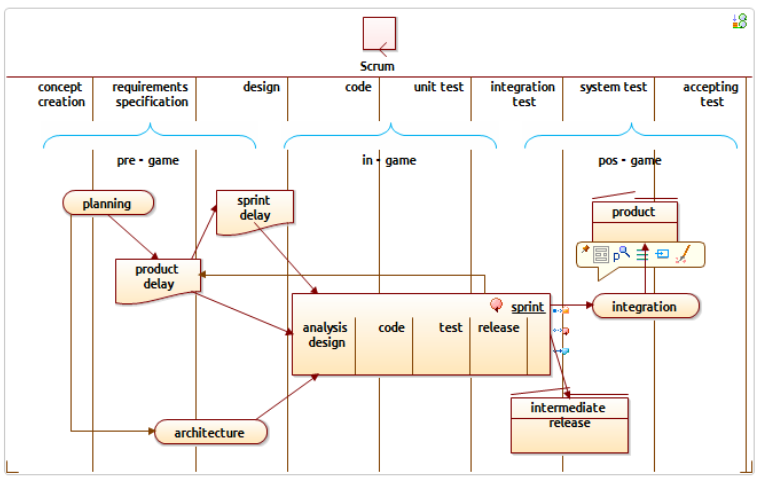
\includegraphics[width=0.6\linewidth]{Scrum}
    \caption{Metodología Scrum}
	\label{fig:Scrum}
\end{figure}
\section{Introducción}
Durante mucho tiempo se buscaron procesos  que se pudieran aplicar en casi cualquier proyecto de desarrollo, los cuales garantizaran la calidad del software y optimizara los tiempos de trabajo, para de esta forma garantizar un producto final de calidad entregado en el plazo de tiempo establecido. El no contar con un proceso de desarrollo puede verse reflejado en el tiempo de producción, ya que este puede ser mucho mayor que el esperado, esto implica igualmente un aumento en los costos.
Las metodologías de desarrollo ágiles surgen debido a la necesidad de generar entregas en el menor tiempo posible, teniendo como prioridad el contacto con el cliente, y la satisfacción de este, para adaptarse de forma rápida al cambio de los requerimientos, del mercado  y a las tecnologías nuevas que se desarrollan, sin dejar de lado la calidad del software en cada entrega.
\newpage
\section{Scrum}
El scrum es un marco de referencia para el desarrollo de software que va de la mano con los principios del manifiesto ágil, el cual busca servir como guía para los procesos de establecer los requerimientos, análisis, diseño, avances y entregas.
Este método fue desarrollado por Jeff Sutherland y su equipo de desarrollo en el año 1990. En años más recientes Schwaber y Beedle han desarrollado más el método Scrum.\cite{Pressman_2010}
En esta metodología el trabajo es dividido en sprints, que por lo general duran dos semanas, pero puede variar dependiendo del tiempo disponible, durante cada sprint se realizan reuniones diarias de por lo general 15 minutos de duración, los cuales sirven para actualizar los avances, informar de los obstáculos que se han presentado y planear lo que se hará hasta la próxima reunión. Esto funciona como estrategia para garantizar que los procesos planteados para el sprint se cumplan.
\newline
\newline
En cada Sprint se incluyen los requerimientos más importantes, los que se van a desarrollar en esa iteración, los cuales están ordenados en una pila de trabajo, en donde las prioridades se encuentran en la parte superior de la pila. Se discute un plan para la realización de los requerimientos, listando las tareas necesarias para estos. Al final de cada sprint se espera que las funcionalidades que entraron estén terminadas y listas para ser presentadas al cliente, se hace también una retrospectiva para evaluar la forma de trabajar del equipo, todos los aspectos a mejorar para la próxima iteración.
\newline
\newline
En la metodología Scrum se cuenta con distintos actores,los cuales tienen un papel importante en el desarrollo del producto:
\newline
\begin{itemize}
	\item Dueño del producto: Esta persona define los requerimientos del producto y es el único que dado el caso puede cambiarlos.
	\item Equipo de trabajo: Son grupos multidisciplinarios y auto-organizados, que trabajan en el desarrollo del producto.
	\item Scrum master o Facilitador: Es una persona externa, preferiblemente, a los grupos de trabajo, la cual dirige los encuentros diarios, ayuda a dar solución a los diferentes problemas que se puedan presentar y evalúa el progreso que tiene cada persona con el fin de conseguir los objetivos de cada iteración.
\end{itemize} 
\newpage
\section{Ventajas y Desventajas}

\subsection{Ventajas}

\begin{itemize}
\item A diferencia de las metodologías tradicionales, el scrum nos permite un desarrollo del proyecto dinámico y ágil, es decir podemos estar enviando entregables al cliente y al mismo tiempo, si es necesario, modificarlo de acuerdo a nuevas especificaciones o necesidades.

\item Permite una mayor eficiencia por parte de cada persona perteneciente al proyecto, esto debido a que cada quien sabe cual es su tarea, es decir requiere de un gran orden para ser aplicado.

\item Da un rol mas incluyente al cliente y a los desarrolladores del software, esto debido a que es más frecuente las pruebas y entregables del software para el perfeccionamiento del mismo.

\item Permite una planeación detallada de los objetivos a alcanzar, por lo que los imprevistos son menos probables a la hora de la codificación. 
\end{itemize} 
\subsection{Desventajas}

\begin{itemize}
\item El hecho de que se le de un rol tan importante a cada miembro del proyecto, puede traer el inconveniente de que alguno de ellos por distintas causas, no pueda cumplir con su tarea, esto implicaría el retraso en el desarrollo o la sobrecarga de trabajo de otros miembros.

\item Muchas veces se puede presentar que no se cumpla con las fechas estipuladas para los entregables, o simplemente que a la hora de presentarlos no se haya logrado un avance significativo.

\item Es necesario excesivas reuniones entre equipo desarrollador y cliente, todo para la verificación y seguimiento del proyecto, ante esto se pueden presentar problemas de disponibilidad.

\item Un error en Pila de Trabajo significaría la carencia de alguna parte esencial del producto, o por el contrario un desperdicio de tiempo y recursos.
\end{itemize} 
\newpage
\section{Cronograma}
\begin{figure}[th!]
	\centering
	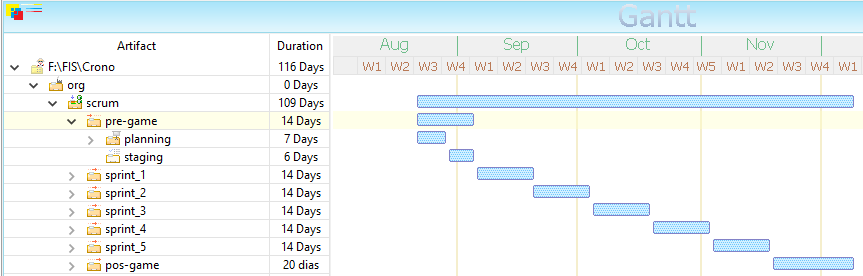
\includegraphics[width=1\linewidth]{Cronograma}
    \caption{Cronograma de la metodología de scrum}
	\label{fig:Cronograma}
\end{figure}
%----------------------------------------------------------------------------------------
%	uml
%----------------------------------------------------------------------------------------
\part{UML}
\chapterimage{banalisis.jpg}
\chapter{Análisis}
\begin{figure}[th!]
	\centering
	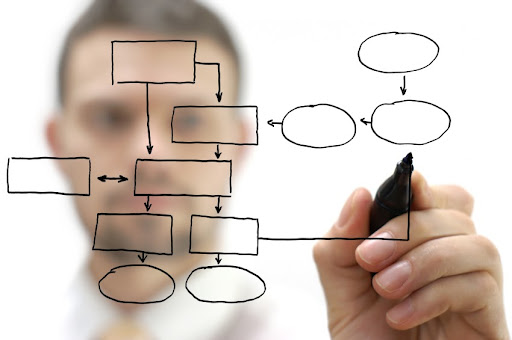
\includegraphics[width=0.4\linewidth]{analisis}
\end{figure}
\section{Introducción}
El análisis de los requerimientos puede ser uno de los procesos más complejos que se presentan a la hora de desarrollar un programa de software, esto se debe a que muchas veces no basta con entender el problema y la posible solución para este, sino que igualmente es necesario comprender las necesidades del cliente, saber qué es lo que quiere, pero muchas veces es el mismo cliente el que no sabe esto último, lo cual complica bastante el proceso.
\newline
\newline
Realizar un buen análisis del proyecto nos garantiza una base solida para la elaboración de nuestro producto, de ahí que sea una de las partes más importante, quizá la más importante, a la hora de realizar un proyecto, ya que es nuestro punto de partida, la forma que tenemos para guiarnos durante el proceso de desarrollo, los planos de nuestro proyecto, por lo que sin el análisis inicial lo más probable es que se este destinado al fracaso.
\newpage

\section{Diagrama de Casos de Uso}

\begin{figure}[th!]
	\centering
	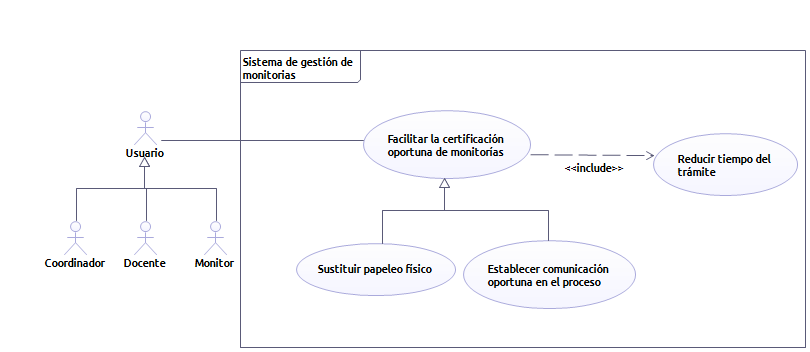
\includegraphics[width=1\linewidth]{Casodeuso}
    \caption{Caso de uso del sistema de gestión de monitorias}
	\label{fig:Casodeuso}
\end{figure}

\begin{table}[H]
\centering
\begin{tabular}{|l|l|l|l|}
\hline
\textbf{Nombre:}        & Sustituir papeleo físico                                                      & \textbf{Id:}                                                    & CU01                                                   \\ \hline
\textbf{Actores:}       & \multicolumn{3}{l|}{Monitor, Profesor}                                                                                                                                                                   \\ \hline
\textbf{Objetivo:}      & \multicolumn{3}{l|}{Agilizar la certificación de la monitoria}                                                                                                                                           \\ \hline
\multicolumn{4}{|c|}{\textbf{Escenarios}}                                                                                                                                                                                          \\ \hline
\textbf{Primario:}      & \multicolumn{3}{l|}{Digitalizar toda la documentación requerida en el proceso}                                                                                                                                 \\ \hline
\textbf{Secundario:}    & \multicolumn{3}{l|}{\begin{tabular}[c]{@{}l@{}}-Documentación incompleta\\ -Horas incompletas\\ -Objetivos incompletos\end{tabular}}                                                                     \\ \hline
\textbf{Excepcionales:} & \multicolumn{3}{l|}{\begin{tabular}[c]{@{}l@{}}-Tamaño virtual de los soportes muy grande \\ -Formato de los soportes incompatible\\ -Falta de comunicación\\ -Inconsistencia en los datos

\end{tabular}} \\ \hline
\end{tabular}
\caption{Especificaciones de caso de uso 01}
\label{tab:EspecificacionCu01}
\end{table}

\begin{table}[H]
\centering
\begin{tabular}{|l|l|l|l|}
\hline
\textbf{Nombre:}        & \begin{tabular}[c]{@{}l@{}}Establecer una comunicación oportuna\\ en el proceso.\end{tabular}                      & \textbf{Id:}                     & CU02                    \\ \hline
\textbf{Actores:}       & \multicolumn{3}{l|}{Monitor, Profesor, Coordinador}                                                                                                                              \\ \hline
\textbf{Objetivo:}      & \multicolumn{3}{l|}{\begin{tabular}[c]{@{}l@{}}Contribuir a la interacción entre los actores del \\ sistema\end{tabular}}                                                        \\ \hline
\multicolumn{4}{|c|}{\textbf{Escenarios}}                                                                                                                                                                  \\ \hline
\textbf{Primario:}      & \multicolumn{3}{l|}{Visualizar la información de contacto de los actores}                                                                                                        \\ \hline
\textbf{Secundario:}    & \multicolumn{3}{l|}{\begin{tabular}[c]{@{}l@{}}-Inexistencia de datos registrados\\ -Información de contacto incompleta\\ -Inconsistencia de los datos de contacto\end{tabular}} \\ \hline
\textbf{Excepcionales:} & \multicolumn{3}{l|}{\begin{tabular}[c]{@{}l@{}}-Fallo en la persistencia de los datos\\ -Falla de comunicación\end{tabular}}                                                     \\ \hline
\end{tabular}
\caption{Especificaciones de caso de uso 02}
\label{tab:EspecificacionCu02}
\end{table}

\begin{table}[H]
\centering
\begin{tabular}{|l|l|l|l|}
\hline
\textbf{Nombre:}        & Reducir tiempo de tramite                                                             & \textbf{Id:}                                                         & CU03                                                         \\ \hline
\textbf{Actores:}       & \multicolumn{3}{l|}{Monitor, Profesor, Coordinador}                                                                                                                                                                         \\ \hline
\textbf{Objetivo:}      & \multicolumn{3}{l|}{Contribuir a la rápida certificación de monitores}                                                                                                                                                      \\ \hline
\multicolumn{4}{|c|}{\textbf{Escenarios}}                                                                                                                                                                                                             \\ \hline
\textbf{Primario:}      & \multicolumn{3}{l|}{\begin{tabular}[c]{@{}l@{}}Generar informe de certificación dentro de fechas\\ preestablecidas\end{tabular}}                                                                                            \\ \hline
\textbf{Secundario:}    & \multicolumn{3}{l|}{-Vencimiento de plazo para la certificación}                                                                                                                                                            \\ \hline
\textbf{Excepcionales:} & \multicolumn{3}{l|}{\begin{tabular}[c]{@{}l@{}}-Falta de oportunidades para completar las horas/\\ objetivos\\ -Retraso en el cumplimiento de las tareas.\\ -Fallas en el calendario del servidor del sistema\end{tabular}} \\ \hline
\end{tabular}
\caption{Especificaciones de caso de uso 03}
\label{tab:EspecificacionCu03}
\end{table}

\newpage

\section{Interacciones}
Todos los sistemas incluyen interacciones de algún tipo. Éstas son interacciones del usuario, que implican entradas y salidas del usuario; interacciones entre el sistema a desarrollar y otros sistemas; o interacciones entre los componentes del sistema. El modelado de interacción del usuario es importante, pues ayuda a identificar los requerimientos del usuario. El modelado de la interacción sistema a sistema destaca los problemas de comunicación que se lleguen a presentar. El modelado de interacción de componentes ayuda a entender si es probable que una estructura de un sistema propuesto obtenga el rendimiento y la confiabilidad requeridos por el sistema.\cite{modeladosistema}

Los diagramas de interacción de más frecuente uso son los siguientes:
\begin{itemize}
\item Diagrama de Secuencia
\begin{figure}[H]
	\centering
	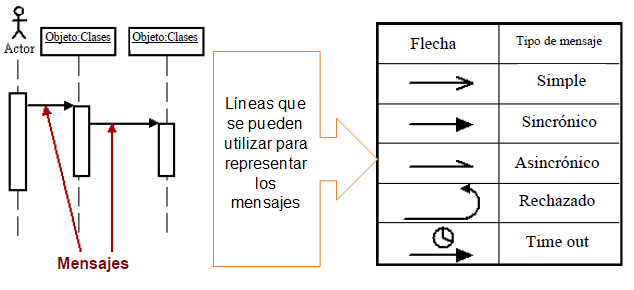
\includegraphics[width=0.7\linewidth]{diagsec}
    \caption{Ejemplo de diagrama de secuencia}
	\label{fig:dseEjemplo}
\end{figure}
\item Diagrama de Comunicación
\begin{figure}[H]
	\centering
	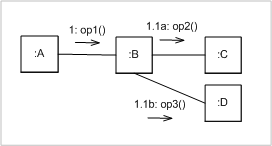
\includegraphics[width=0.7\linewidth]{diagcom}
    \caption{Ejemplo de diagrama de comunicaciones}
	\label{fig:dcomEjemplo}
\end{figure}
\end{itemize}
\newpage
\subsection{Diagrama de Secuencia}
El diagrama de secuencia es un tipo de diagrama usado para modelar interacción entre objetos
en un sistema. Este tipo de diagrama muestra la interacción de un conjunto de objetos en una aplicación
a través del tiempo y se modela para cada caso de uso. Mientras que el diagrama de casos de uso
permite el modelado de una vista del negocio para el escenario, el diagrama de secuencia contiene detalles
de implementación del escenario, incluyendo los objetos y clases que se usan para implementar el
escenario y mensajes intercambiados entre los objetos.

A continuación se muestran algunos de los escenarios más importantes de las interacciones del sistema:
\begin{figure}[th!]
	\centering
	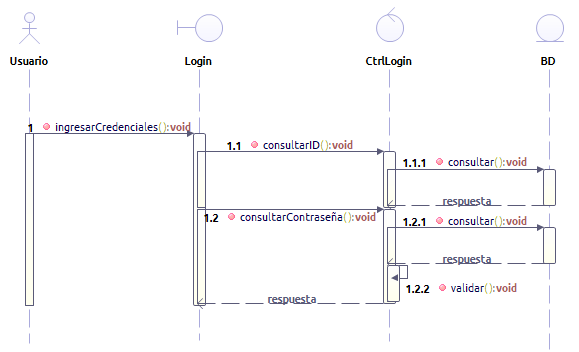
\includegraphics[width=1\linewidth]{patronlogueo}
    \centering
    \caption{Diagrama de secuencia para la autenticación de un usuario en el sistema}
	\label{fig:patronlogueo}
\end{figure}

En el anterior diagrama de secuencia sucede lo primero que debe hacer un usuario antes de hacer uso de las funcionalidades del sistema: autenticarse como un usuario, este usuario es único y tiene distintas funcionalidades dependiendo de su rol. 
\clearpage
Por ejemplo en el siguiente diagrama de secuencia se muestra la funcionalidad del escenario primario del caso de uso 03 apreciado en el cuatro 3.3, donde el coordinador se encarga de generar los certificados de cada monitor.

\begin{figure}[H]
	\centering
	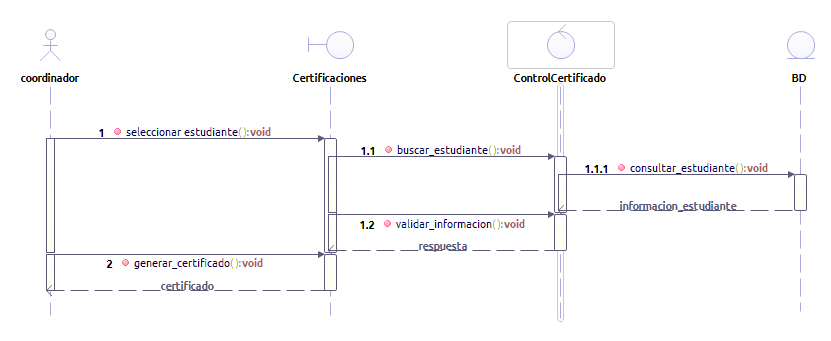
\includegraphics[width=1\linewidth]{diagseqcertificado}
    \caption{Diagrama de secuencia para la certificación de las monitorías}
	\label{fig:dsecertificacion}
\end{figure}

Por otro lado una funcionalidad clave del sistema es permitir el contacto oportuno entre los usuarios del sistema, observado en el caso de uso 02 del cuadro 3.2. En este diagrama de secuencia se generaliza primordialmente para todos los usuarios, pues todos tienen la posibilidad de visualizar bien sea el correo o el teléfono de los involucrados en el proceso.
\begin{figure}[H]
	\centering
	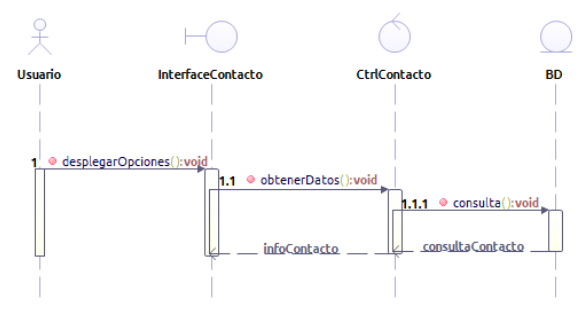
\includegraphics[width=1\linewidth]{dsecontacto}
    \caption{Diagrama de secuencia para el contacto entre usuarios del sistema}
	\label{fig:dsecontacto}
\end{figure}

Ahora, existirán situaciones en las que un docente necesita de ayuda extra dentro de la academia, y un estudiante necesita horas para poder certificarse, es en este escenario donde el docente puede publicar un clasificado en el sistema a la espera de que algún estudiante lo contacte, a continuación se visualiza esta situación en un diagrama de secuencia: 
\begin{figure}[H]
	\centering
	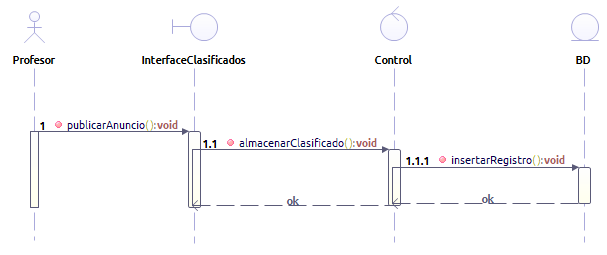
\includegraphics[width=1\linewidth]{dseclasificados}
    \centering
    \caption{Diagrama de secuencia para la publicación de clasificados por parte del profesor}
	\label{fig:dseclasificados}
\end{figure}

En el siguiente diagrama de secuencia puede que describamos uno de los procesos más fundamentales de nuestro aplicativo, el hecho de permitirle a el docente poder llevar un registro de las horas de los monitores a su cargo es algo esencial, por ello nuestro actor principal en esta abstracción sera el docente, aquel que tiene acceso a una interfaz gráfica que le luego le permitirá seleccionar a un estudiante, por medio de una petición la interfaz accede  al control para que este posteriormente, pueda acceder a la base de datos de los estudiantes y pueda regresar información sobre las horas de monitoria de un estudiante, al obtener esta información en un proceso inmediatamente continuo, se desplegara en la interfaz esta información, para que el docente pueda modificarla, es decir para que el docente tenga la capacidad de llenar las horas que le hacen falta al estudiante. De este modo nos aseguramos de una total transparencia en el proceso, ademas de el hecho de ahorrarnos un montón de papeleo y firmas innecesarias:
\begin{figure}[H]
	\centering
	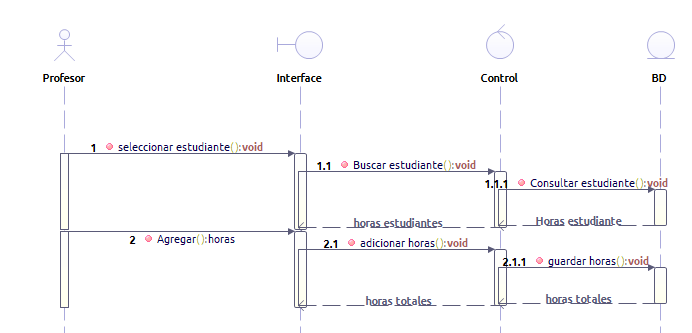
\includegraphics[width=1\linewidth]{horas}
    \centering
    \caption{Diagrama de secuencia para la certificación de horas de monitoría}
	\label{fig:dsehoras}
\end{figure}

El diagrama de digitalización de los documentos nos describe una automatización y visualización virtual, completa de los documentos que se tienen que presentar en los procesos de monitorias, para ello haremos uso de una base de datos que lleve registro de cada uno de los estudiantes implicados en las monitorias, como es obvio nuestro actor principal sera el estudiante, para ser exactos los monitores, ellos podrán acceder a la plataforma mediante sus cuentas, en donde encontraran una interfaz que les permitirá llenar su información principal y donde podrán subir todo documento requerido, para ello deberán subir una imagen de dichos requisitos, la cual sera llevada a un control que procederá a guardar la en la base de datos, si no hay errores externos, la plataforma le verificara al estudiante el estado de su  información:
\begin{figure}[H]
	\centering
	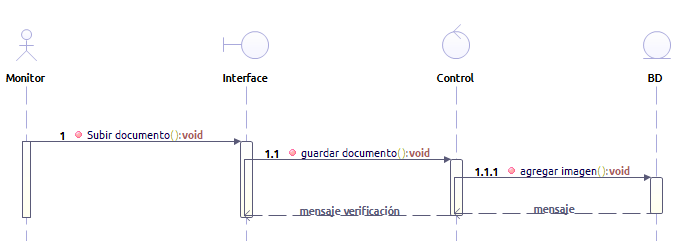
\includegraphics[width=1\linewidth]{digidoc}
    \centering
    \caption{Diagrama de secuencia para la digitalización de documentos}
	\label{fig:dsedigidoc}
\end{figure}


\newpage

\subsection{Diagrama de Comunicación}
Un diagrama de comunicación nos permite modelar las distintas interacciones y acciones entre objetos de nuestro proyecto, normalmente son combinaciones de información de otro tipo de diagramas tales como el de clases o el de secuencia que previamente hemos realizado, este nos ayuda a describir el comportamiento de nuestro sistema por medio de mensajes, por ello es normal que el nombre de los objetos del diagrama de comunicación sean los mismo que los del diagrama de secuencia, estos mensajes al igual que en el anterior diagrama están organizados por importancia a la hora de ser realizados, no podemos acceder a una base de datos si previamente no nos identificamos con el sistema.

En el siguiente diagrama de comunicación podemos ver el proceso del sistema a la hora de ingresar al sistema, pero podemos observar un cambio en el control  al acceso de la base de datos, como podemos ver en este objeto tenemos un mensaje que esta redireccionando a si mismo, es decir que este tiene la capacidad de validar antes de devolver la información a la interfaz, esto es esencial en aplicativo debido a que si no pensáramos en este tipo de control, en un nivel alto de nuestra aplicación cualquiera podría acceder a los datos y dañar nuestra información. 

\begin{figure}[H]
	\centering
	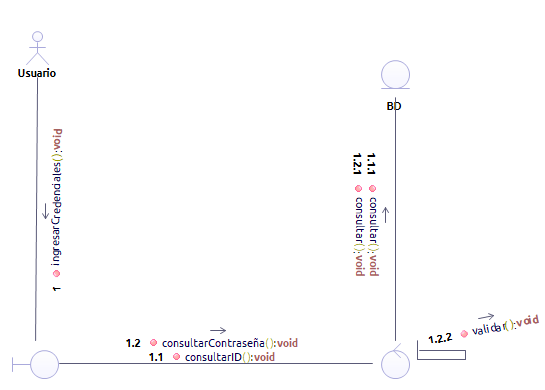
\includegraphics[width=0.8\linewidth]{dcomLogin}
    \centering
    \caption{Diagrama de comunicación para el diagrama de secuencia de la figura 3.2}
	\label{fig:dcomLogin}
\end{figure}
\clearpage
Cada doble mensaje que observamos nos permite visualizar una acción que toma nuestro sistema, aun y sin embargo este diagrama no nos permite visualizar los mensajes de retorno, esto se debe a que estos diagramas de comunicación son un complemento de nuestro proceso de abstracción, en este caso nos retornaría la información del estudiante. 
\begin{figure}[H]
	\centering
	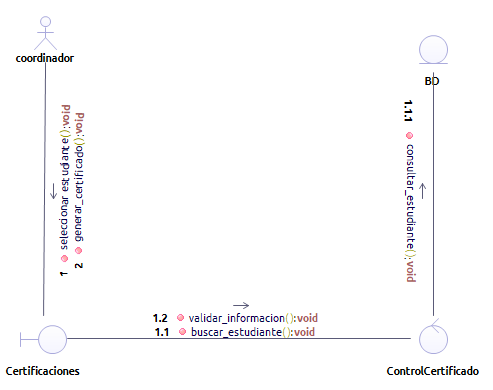
\includegraphics[width=0.8\linewidth]{dcomCertifi}
    \centering
    \caption{Diagrama de comunicación para el diagrama de secuencia de la figura 3.3}
	\label{fig:dcomCertifi}
\end{figure}
\clearpage
El siguiente diagrama de comunicación refleja la secuencia de mensajes realizada por el programa para permitir al usuario obtener la información necesaria, en este caso la información de contacto de otro usuario, que puede ser profesor o monitor y con lo que se garantizaría la oportuna comunicación entre los diferentes usuarios de la aplicación. 
\begin{figure}[H]
	\centering
	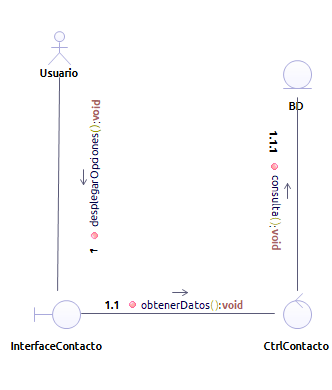
\includegraphics[width=0.8\linewidth]{dcomContacto}
    \centering
    \caption{Diagrama de comunicación para el diagrama de secuencia de la figura 3.6}
	\label{fig:dcomContacto}
\end{figure}
\clearpage
Del mismo modo la siguiente figura ilustrar la forma en la que el programa permite a un docente buscar un monitor disponible, por medio de un clasificado que será guardado y posteriormente mostrado a los demás usuarios, específicamente a los monitores que estén disponibles para completar sus horas de monitoria.
\begin{figure}[H]
	\centering
	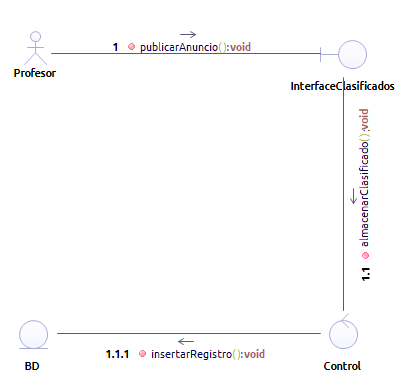
\includegraphics[width=0.8\linewidth]{dcomClasifi}
    \centering
    \caption{Diagrama de comunicación para el diagrama de secuencia de la figura 3.7}
	\label{fig:dcomClasifi}
\end{figure}
\clearpage
El siguiente diagrama de comunicación nos da a conocer las direcciones de los mensajes entre los distintos objetos, desde el profesor y seleccionar a un estudiante y agregarle las horas correspondientes por su labor de monitorias, lo cual lo realiza mediante un objeto interface, este nos permite representar la parte grafica de nuestra app, a su vez conectado por un objeto control, este se encarga de transmitir la información capturada en el objeto que interactúa con el actor principal, haciendo las veces de puente entre una interface y una persistencia, este referencia la información a nuestro objeto base de datos (BD) este realiza la función de consulta y modificación de la base, mediante los mensajes de consultar datos del estudiante y guardar las horas.
\begin{figure}[H]
	\centering
	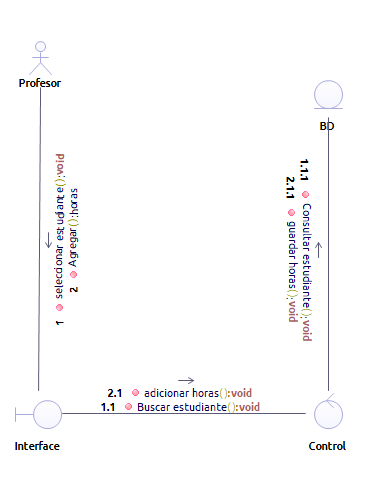
\includegraphics[width=0.7\linewidth]{dcomHoras}
    \centering
    \caption{Diagrama de comunicación para el diagrama de secuencia de la figura 3.6}
	\label{fig:dcomHoras}
\end{figure}
\clearpage
Este diagrama de comunicación es el que nos permite la virtualización en gran parte del papeleo, para ello el actor principal en este caso un estudiante, al llenar su información personal, junto con algunos archivos específicos e imágenes, interactúa con un objeto Interface, aquel le permite al usuario digitar y capturar sus datos para evitar todo tramite presencial y molesto, mediante el mensaje subir documento, se planea capturar toda información de un estudiante para luego ser llevada a un control que se encargue mediante otro enlace de comunicación de decirle al objeto BD, que es el que interactúa directamente con nuestra base de datos, que actualice cierta información, dado cierto punto del proceso, el actor solo podrá actualizar su información, ya que la modificación de sus datos personales solo será supervisada por un actor externo de mayor jerarquía, esto con el fin de evitar información corrupta
\begin{figure}[H]
	\centering
	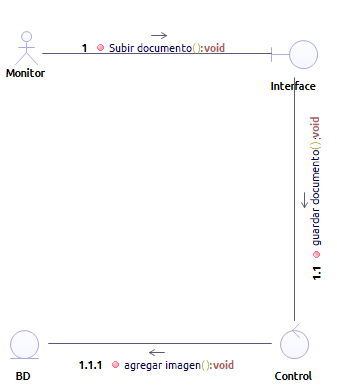
\includegraphics[width=0.7\linewidth]{dcomDigi}
    \centering
    \caption{Diagrama de comunicación para el diagrama de secuencia de la figura 3.7}
	\label{fig:dcomDigi}
\end{figure}
\clearpage

\newpage

\subsection{Diagrama de Temporización}

\newpage

\section{Diagramas de Actividades}
Este tipo de diagramas muestran el flujo de actividades de un proceso de negocio o un proceso de software por medio de un conjunto de actividades que principalmente son realizadas por componentes de software. Los diagramas de actividades permiten ver la secuencia de mensajes o interacciones que se realiza entre entidades.
Dentro del Sistema de Gestión de Monitorias se destacan los siguientes diagramas:

\begin{figure}[H]
	\centering
	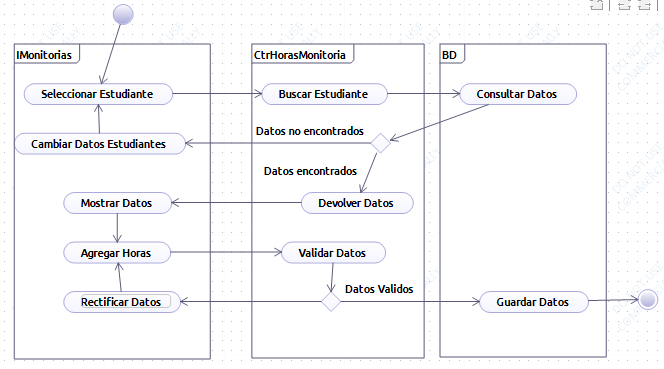
\includegraphics[width=0.9\linewidth]{actCertificarHoras}
	\centering
	\caption{Diagrama de actividades para la certificación de horas.}
	\label{fig:actCertificarHoras}
\end{figure}

\begin{figure}[H]
	\centering
	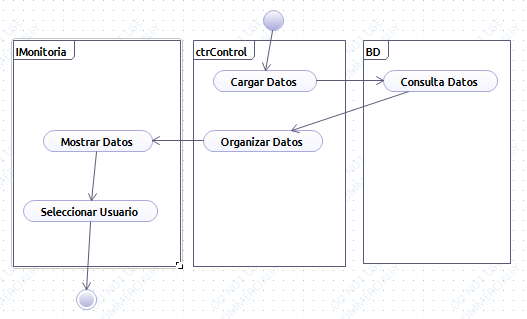
\includegraphics[width=0.9\linewidth]{actContacto}
	\centering
	\caption{Diagrama de actividades para el proceso de contactar otro usuario.}
	\label{fig:actContacto}
\end{figure}

\begin{figure}[H]
	\centering
	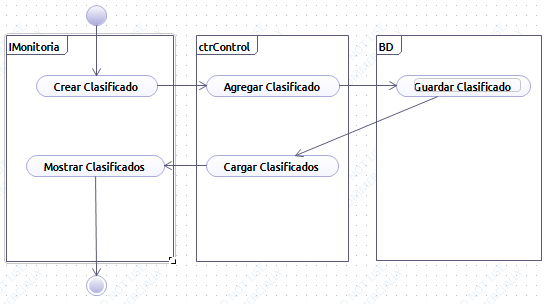
\includegraphics[width=0.9\linewidth]{actClasificados}
	\centering
	\caption{Diagrama de actividades para el proceso de publicar una clasificado.}
	\label{fig:actClasificados}
\end{figure}
\newpage
\newpage

\section{Diagramas de Workflow}

Workflow es la automatización de un proceso de negocio, sea parcial o totalmente, durante el cual documentos, información o tareas son pasados desde un participante a otro para la ejecución de otra acción, de acuerdo a un conjunto de reglas procedurales. \cite{workflow} Para el caso del Sistema de Gestión de Monitorías se pueden destacar los siguientes procesos:

\begin{figure}[H]
	\centering
	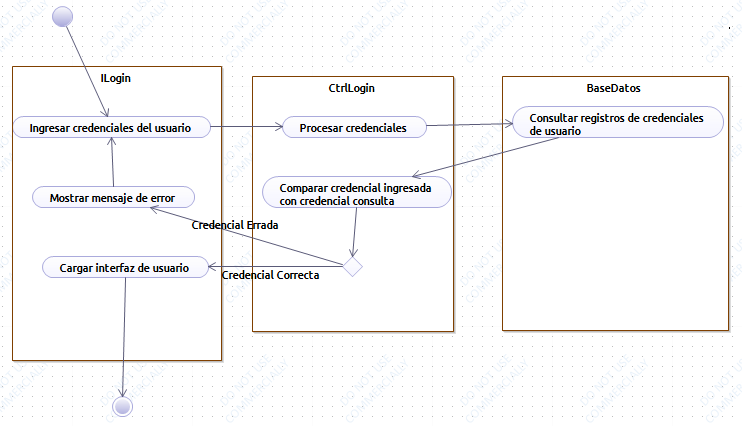
\includegraphics[width=0.9\linewidth]{wfLogin}
	\centering
	\caption{Diagrama de workflow para la autenticación de usuarios.}
	\label{fig:wfLogin}
\end{figure}

\begin{figure}[H]
	\centering
	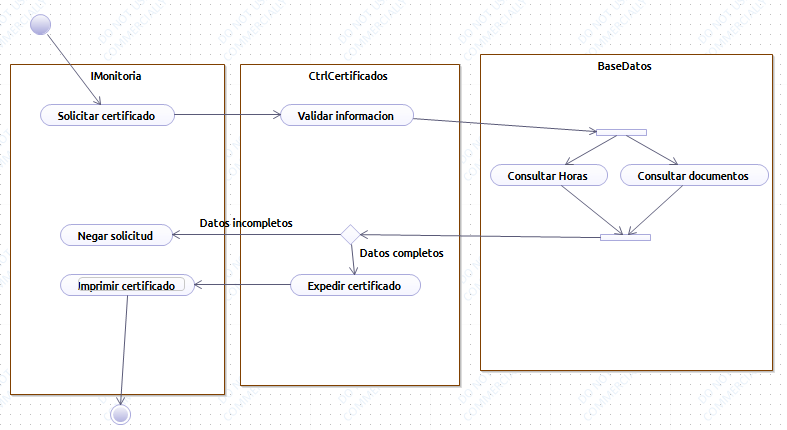
\includegraphics[width=0.9\linewidth]{wfCertificado}
	\centering
	\caption{Diagrama de workflow para la certificación de monitorias.}
	\label{fig:wfCertificado}
\end{figure}
\clearpage
\begin{figure}[H]
	\centering
	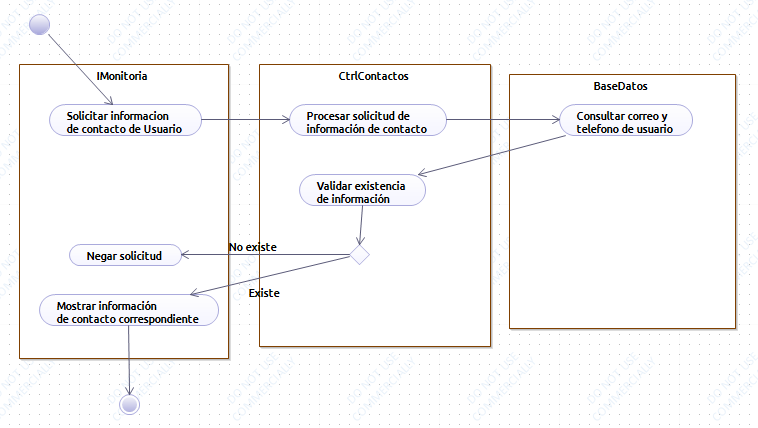
\includegraphics[width=0.9\linewidth]{wfContacto}
	\centering
	\caption{Diagrama de workflow para el contacto de usuarios.}
	\label{fig:wfContacto}
\end{figure}

\newpage

\section{Diagramas de Descripción de la Interacción}

\newpage
\chapterimage{bdiseno.jpg}
\chapter{Diseño}
\begin{figure}[H]
	\centering
	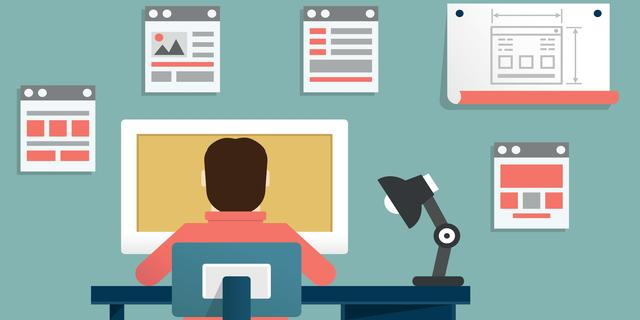
\includegraphics[width=1\linewidth]{diseno}
    \centering
\end{figure}
\section{Introducción}

El diseño del software, constituye una de las bases más importantes a la hora de crear nuevos sistemas. Hoy en día la complejidad creciente del software hace que el riesgo de construir sistemas que no alcancen los objetivos sea muy alto. Para evitar ese riesgo conviene construirlo a partir de una buena fase de planificación mediante diagramas UML que permitan cumplir las expectativas tanto del desarrollador como las del cliente. A continuación se presentarán algunos de los diagramas más importantes relacionados con el diseño del sistema de gestión de monitorías.

\newpage

\section{Diagrama de Clases de Análisis}

Los diagramas de clases de análisis facilitan la realización de los casos de uso del sistema y sirve como una simplificación del modelo de diseño. Entre los 3 elementos que se visualizan en estos diagramas se encuentran la Interfaz, qué es una clase estereotipada la cual describe la realización de los casos de uso del sistema. El otro elemento es el controlador, donde se plasma la lógica del negocio y el último elemento es la entidad, donde se encuentra la persistencia del sistema. 

A continuación se muestra el diagrama de clases de análisis para la parte de la autenticación del usuario.
\begin{figure}[H]
	\centering
	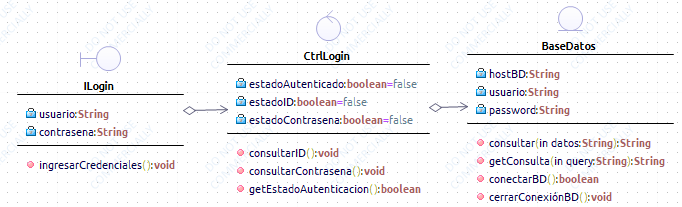
\includegraphics[width=1\linewidth]{dcaLogin}
	\centering
	\caption{Diagrama de Clases de análisis para el Login de la plataforma.}
	\label{fig:dClaALogin}
\end{figure}

Por otro lado se tiene para la certificación de monitorías el siguiente diagrama:

\begin{figure}[H]
	\centering
	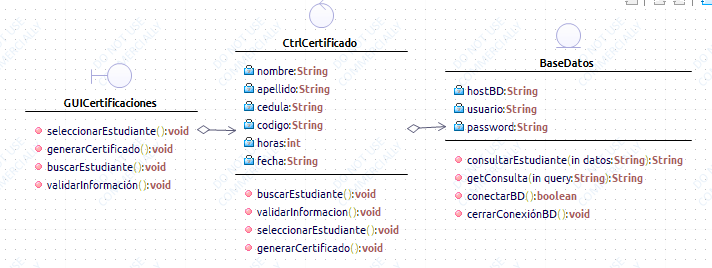
\includegraphics[width=1\linewidth]{dcaCertificacion}
	\centering
	\caption{Diagrama de Clases de análisis para la certificación de monitoría.}
	\label{fig:dcaCertificacion}
\end{figure}
\clearpage
La siguiente figura representa el diagrama de clases de análisis de el contacto entre monitor y profesor

\begin{figure}[H]
	\centering
	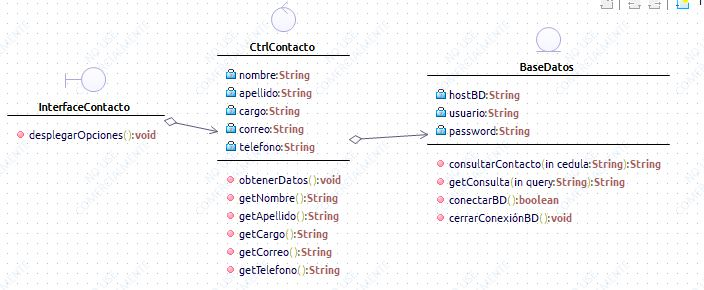
\includegraphics[width=1\linewidth]{dcaContacto}
	\centering
	\caption{Diagrama de Clases de análisis para el contacto Docente-Monitor.}
	\label{fig:dcaContacto}
\end{figure}

En el próximo diagrama de clases de análisis se puede observar las clases que interfieren en el proceso de publicar clasificados.

\begin{figure}[H]
	\centering
	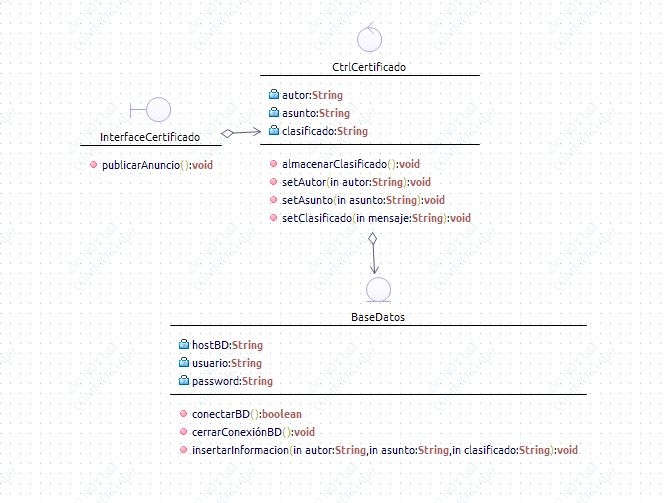
\includegraphics[width=1\linewidth]{dcaClasificados}
	\centering
	\caption{Diagrama de Clases de análisis para el proceso de publicar clasificados .}
	\label{fig:dcaClasificado}
\end{figure}
\clearpage
Por último se tiene el diagrama de clases de análisis de la certificación de las horas de las monitorías.

\begin{figure}[H]
	\centering
	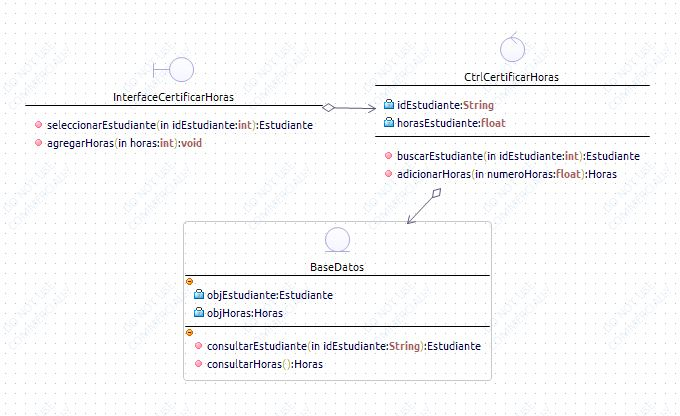
\includegraphics[width=1\linewidth]{dcaCertificarHoras}
	\centering
	\caption{Diagrama de Clases de análisis para el proceso de certificación de horas.}
	\label{fig:dcaCertificarHoras}
\end{figure}

\newpage

\section{Diagrama de Clases}

Un diagrama de clases describe los tipos de objetos que hay en el sistema y las diversas clases de relaciones estáticas que existen entre ellos.
Es importante identificar las relaciones entre las clases. El nombre de la asociación debe dejar claro que una entidad utiliza a otra clase como parte de sus atributos o características. Se debe tener en cuenta que entre dos clases puede existir más de una relación.\cite{Sergio_2015}
\newline
De acuerdo a los diagramas de secuencia y objetos, se realizó una construcción de los diagramas de clase de acuerdo con la utilidad que tiene coloso, a partir de las clases generadas se procedió a editar cada una de estas clases, agregando una serie de atributos y métodos que en un principio se consideran necesario.

El primer diagrama consiste en las clases que administran la forma de ingresar a la plataforma:

\begin{figure}[H]
	\centering
	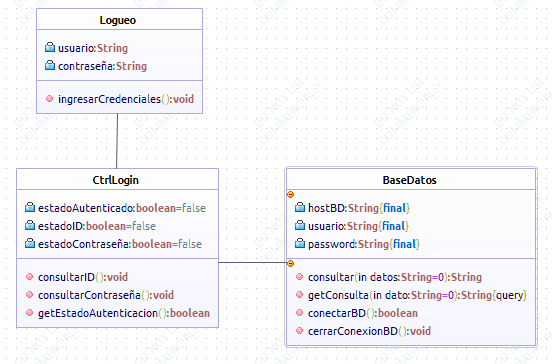
\includegraphics[width=0.8\linewidth]{dclogin}
    \centering
    \caption{Diagrama de Clases para el Login de la plataforma.}
	\label{fig:dClaLogin}
\end{figure}

\newpage
Ahora, en la siguiente imágen se muestra el diagrama de clases para la generación de certificados, en este diagrama la clase control depende de la clase de base de datos para ejecutar su lógica y ésta a su vez usa de una interfaz gráfica donde el usuario interactúa con el aplicativo y este visualiza los datos entregados.

\begin{figure}[H]
	\centering
	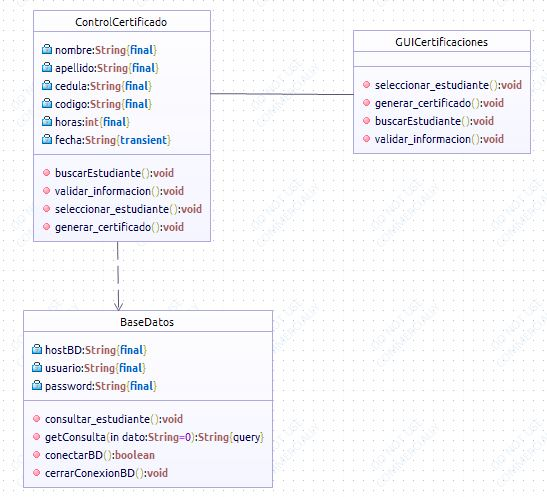
\includegraphics[width=0.8\linewidth]{DiagramaClases}
    \centering
    \caption{Diagrama de Clases para la generación de certificados monitoria.}
	\label{fig:dClaCertificado}
\end{figure}

\newpage
Manera similar sucede con el diagrama de clases para la visualización de contactos, cuya finalidad es obtener unicamente los datos de contacto de los usuarios.
\begin{figure}[H]
	\centering
	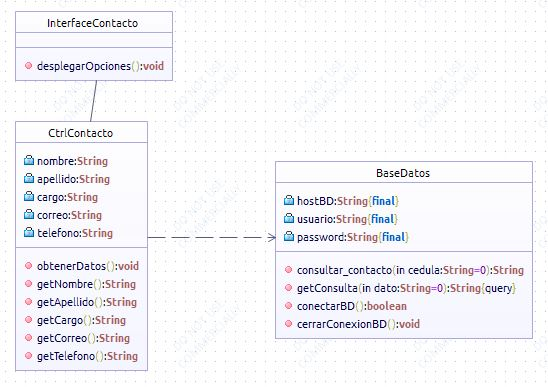
\includegraphics[width=1\linewidth]{dcContacto}
    \centering
    \caption{Diagrama de clases para la visualización de contactos.}
	\label{fig:dClaContacto}
\end{figure}
\newpage
\clearpage
Uno de los beneficios que ofrece la plataforma de gestión de monitorías es el uso de clasificados por parte de los profesores para completar las horas requeridas por el monitor, en base al diagrama de secuencia de la figura 3.7 se propone el siguiente diagrama de clases:

\begin{figure}[H]
	\centering
	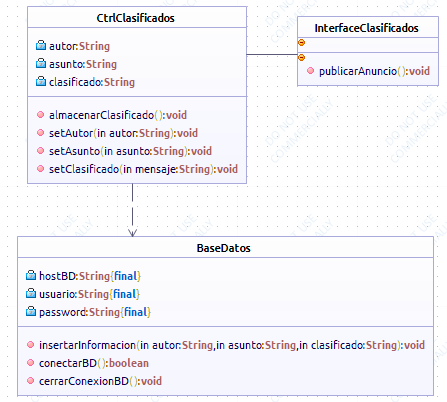
\includegraphics[width=0.8\linewidth]{dcClasificado}
    \centering
    \caption{Diagrama de clases para la publicación de clasificados}
	\label{fig:dClaClasificado}
\end{figure}
\clearpage
La certificación de las horas de monitoria es uno de los procesos imprscindibles en el desarrollo del proyecto, puesto que con este se busca aportar al cumplimiento de varios requerimientos, como los de eliminar el papeleo y facilitar el proceso de certificación, por lo que es importante hacer una correcta espicificación de este.
\begin{figure}[H]
	\centering
	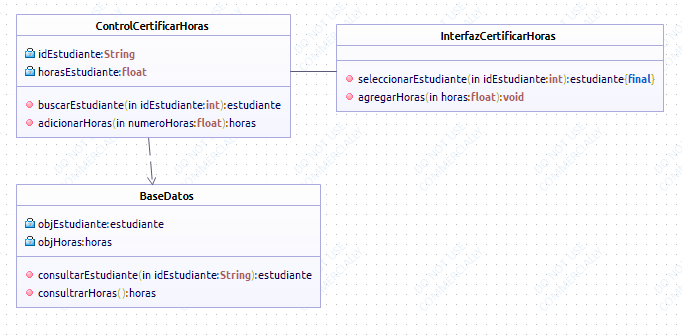
\includegraphics[width=1\linewidth]{dcCertifi}
    \centering
    \caption{Diagrama de clases para la certificación de horas de monitoría}
	\label{fig:dClaCertifi}
\end{figure}

\section{Diagrama de Objetos}

\newpage

\section{Diagrama de Estructura Compuesta}

\newpage

\section{Patrones}
Según Gamma en su libro Patrones de Diseño, define a un patrón de diseño como una descripción
de clases y objetos comunicándose
entre sí adaptada para resolver un
problema de diseño general en un
contexto particular. Con los patrones de diseño es posible saber cual fue la intencionalidad con la que se desarrolló una aplicación y cual será a futuro la intención con la que se desarrolla en el presente. El patrón de diseño no es sólo una plantilla para reusar; es todo un idioma de diseño que estandariza la forma de diseñar aplicaciones, garantizando su fácil evolución, prueba y mantenimiento\cite{Bol_2014}.

Existen 3 tipos de patrones:
\begin{itemize}
\item Creacionales: 
\item Estructurales
\item De comportamiento
\end{itemize}
\subsection{Patrones creacionales}
Los patrones creacionales proporcionan ayuda a la hora de crear instancias de objetos. El objetivo
de este tipo de patrones es el de abstraer el proceso de instanciación y ocultar los detalles de cómo los objetos
son creados o inicializados \cite{Bol_2014}.
Dentro de los patrones creacionales se pueden encontrar los siguientes:
\begin{enumerate}
\item Método Fábrica
\item Fábrica Abstracta
\item Prototype
\item Constructor
\item Singleton
\end{enumerate}

Para el caso concreto de nuestro proyecto, se hará uso del patrón creacional singletón. Por lo que sólo se hará énfasis profundo en éste patrón.
\newpage
\paragraph{Singleton}
El patrón Singleton, también conocido como instancia única, nos permite tener un controlar en número de instancias de un objeto, en este caso, como su nombre lo indica, defina la creación de una única instancia.
\newline
\indent\textbf{Estructura}
\newline
\begin{figure}[H]
	\centering
	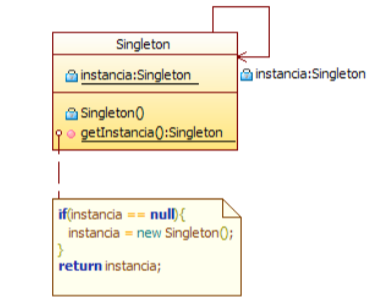
\includegraphics[width=0.5\linewidth]{estructuraSingleton}
    \centering
    \caption{Estructura del patrón Singleton.}
	\label{fig:eSingleton}
\end{figure}
\indent\textbf{Caso de estudio}
\newline
\begin{figure}[H]
	\centering
	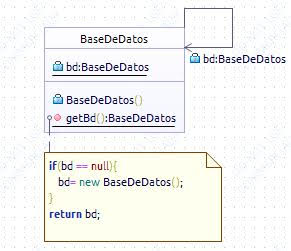
\includegraphics[width=0.5\linewidth]{singleton}
    \centering
    \caption{Singleton del sistema de gestión tutoríaas.}
	\label{fig:singleton}
\end{figure}

\indent Dentro del diseño del aplicativo es necesario garantizar que la base de datos de la que se hace uso sea la misma en todo el aplicativo y que no se creen multiples instancias de esta, por lo que se hará uso del patrón de diseño Singleton para garantizar una única instancia de la base de datos y que esta sea utilizada en todo el aplicativo. Podrá observar un ejemplo de su implementación en el anexo 8.1.1.
\newpage
\subsection{Patrones Estructurales}
Los patrones estructurales se enfocan en como las clases y objetos se componen para formar
estructuras mayores, los patrones estructurales describen como las estructuras compuestas por clases
crecen para crear nuevas funcionalidades de manera de agregar a la estructura flexibilidad y que la
misma pueda cambiar en tiempo de ejecución lo cual es imposible con una composición de clases
estáticas\cite{estruct}.
Dentro de los patrones estructurales se pueden encontrar los siguientes:
\begin{enumerate}
\item Puente
\item Adaptador
\item Componente
\item Decorador
\item Fachada
\item Peso Ligero
\item Proxy
\end{enumerate}

Para el caso concreto de nuestro proyecto, se hará uso de los patrones estructurales Componente, Fachada y Proxy. Por lo que sólo se hará énfasis profundo en estos patrones.
\paragraph{Patrón Fachada}
\indent El patrón fachada provee una interface unificada para un conjunto de interfaces en un subsistema, la fachada es una interface de alto nivel que facilita el uso de un subsistema. Su uso principal consiste en la posibilidad de crear un sistema de niveles\cite{Bol_2014}.
\newline
\indent\textbf{Estructura}
\newline
\begin{figure}[H]
	\centering
	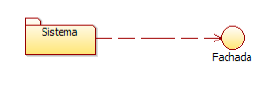
\includegraphics[width=0.5\linewidth]{fachada}
    \centering
    \caption{Estructura del patrón fachada.}
	\label{fig:eFachada}
\end{figure}
\indent\textbf{Caso de estudio}
\begin{figure}[H]
	\centering
	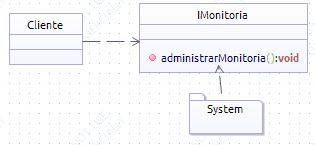
\includegraphics[width=0.5\linewidth]{dcFachada}
    \centering
    \caption{Fachada del sistema de gestión de tutorías.}
	\label{fig:dcFachada}
\end{figure}
\indent Para el diseño del aplicativo de gestión de monitorías se utilizará una fachada que reuna las implementaciones más fundamentales con las que el usuario interactuará. Desacoplando la implementación del cliente con todo el subsistema y simplificando su uso. Puede observar un ejemplo de su implementación en el Anexo 8.1.2.
\newpage
\paragraph{Patrón Componente}
El patrón componente simplifica el uso de varios objetos similares organizandolos en una estructura tipo árbol que representa el todo-parte\cite{Bol_2014}, lo cual simplifica la creación de algoritmos y objetos complejos haciendo uso de la recursión al tratar al todo igual que a una parte.
\begin{figure}[H]
	\centering
	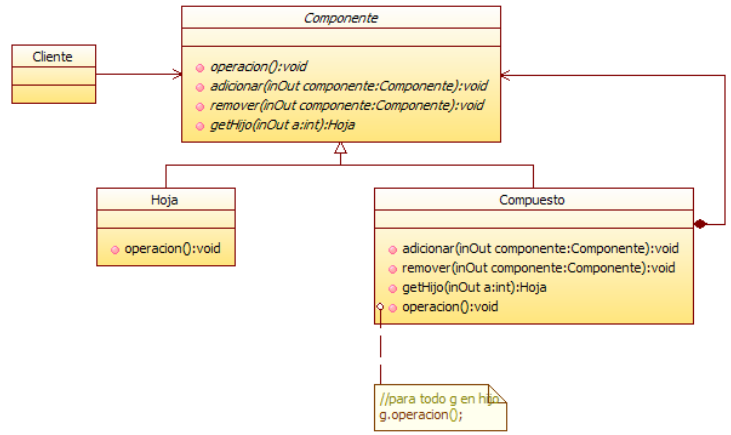
\includegraphics[width=0.8\linewidth]{PatronComponente}
    \centering
    \caption{Estructura del patrón componente.}
	\label{fig:eComponente}
\end{figure}
\indent\textbf{Caso de estudio}
\newline
\begin{figure}[H]
	\centering
	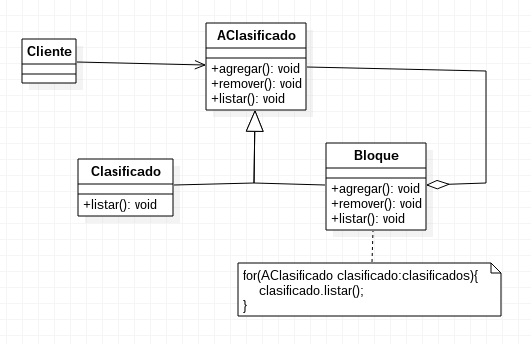
\includegraphics[width=0.6\linewidth]{composite}
    \centering
    \caption{Patrón componente del sistema de gestión de tutorías..}
	\label{fig:composite}
\end{figure}
\indent Dentro de la aplicación de monitorias se creará una zona de clasificados en donde los monitores podrán observar las publicaciones hechas por los profesores que requieran de sus servicios. Para el manejo de estos clasificados se ha decidido hacer uso del patrón componente, el cual permite agrupar los clasificados en una estructura en forma de árbol, lo que permite hacer uso de la recursión para facilitar la forma en la que se van a visualizar los clasificados. Podrá observar un ejemplo de su implementación en el anexo 8.1.3. 
\newpage
\paragraph{Patrón Proxy}
Provee un sustituto o marcador para otro objeto que controla el acceso a él. Controla el acceso a un objeto o lo representa localmente o por su alta demanda.\cite{Bol_2014}.
\newline
\indent\textbf{Estructura}
\newline
\begin{figure}[H]
	\centering
	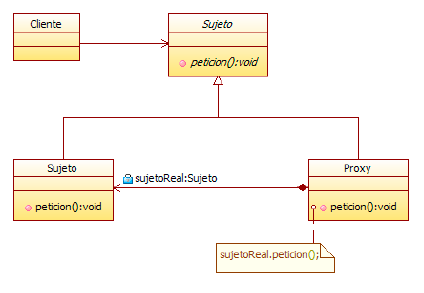
\includegraphics[width=0.5\linewidth]{proxyestruct}
    \centering
    \caption{Estructura del patrón proxy.}
	\label{fig:eProxy}
\end{figure}
\indent\textbf{Caso de estudio}
\begin{figure}[H]
	\centering
	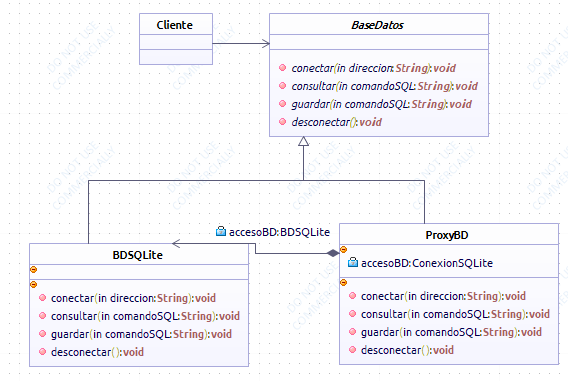
\includegraphics[width=0.5\linewidth]{dcProxy}
    \centering
    \caption{Implementación del patrón proxy.}
	\label{fig:dcProxy}
\end{figure}
\indent El patrón Proxy actúa en el diseño del sistema de gestión de monitorías como intermediario para poder realizar operaciones en la base de datos SQLite, el proxy recibe la solicitud de alguna operación en la base de datos, y si es posible hacerla se delegan las funciones a la clase BDSQLite, caso contrario no se ejecuta ninguna acción lo cual reduce el uso de recursos. Podrá observar un ejemplo de su implementación en el anexo 8.1.4.
\newpage
\subsection{Patrones de Comportamiento}
Los patrones de comportamiento explican la forma en la que los objetos interactúan entre sí. Describe como los diferentes objetos y clases intercambian mensajes entre ellos para hacer que las cosas funcionen y describir como los pasos de una tarea en específico es dividida a lo largo de distintos objetos. A diferencia de los patrones creacionales que solo describen el momento en que se crean los objetos y los patrones estructurales que describen una estructura más o menos estática, los patrones de comportamiento describen un proceso o flujo de información\cite{behavioral}.
Dentro de los patrones de comportamiento se pueden encontrar los siguientes:
\begin{enumerate}
\item Cadena de Responsabilidad
\item Comando
\item Interprete
\item Iterador
\item Mediador
\item Momento
\item Observador
\item Estado
\item Estrategia
\item Método Plantilla
\item Visitador
\end{enumerate}

Para el caso concreto de nuestro proyecto, se hará uso del patrón de comportamiento comando. Por lo que sólo se hará énfasis profundo en éste patrón.
\paragraph{Patrón Comando}
El patrón comando nos permite encapsular una petición en un objeto, es decir que nos permite parametrizar a los clientes con diferentes peticiones, esto significa que podemos hacer peticiones a objetos de nuestra aplicación sin ser especificados, este es un método importante, debido a que como desarrolladores muchas veces no tenemos modo de conocer al receptor de la petición, ni de saber que operaciones se efectuaran, en términos conceptuales este patrón nos permite asegurar el encapsulamiento y por ende la seguridad de nuestra información
\newline
\indent\textbf{Estructura}
\begin{figure}[H]
	\centering
	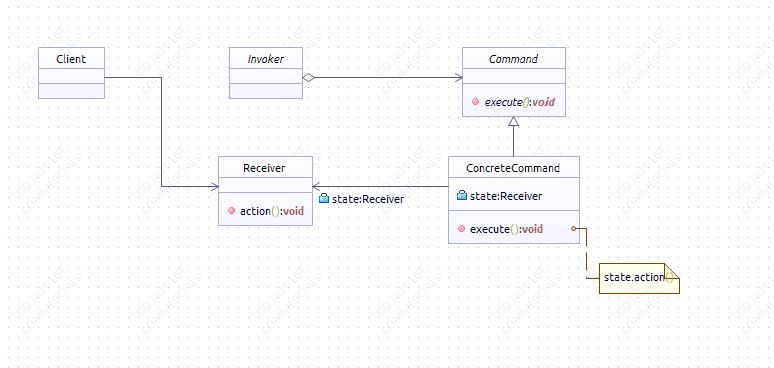
\includegraphics[width=0.8\linewidth]{mComando}
    \centering
    \caption{Estructura general del patron comando.}
	\label{fig:mComando}
\end{figure}
\clearpage
\indent\textbf{Caso de estudio}
\begin{figure}[H]
	\centering
	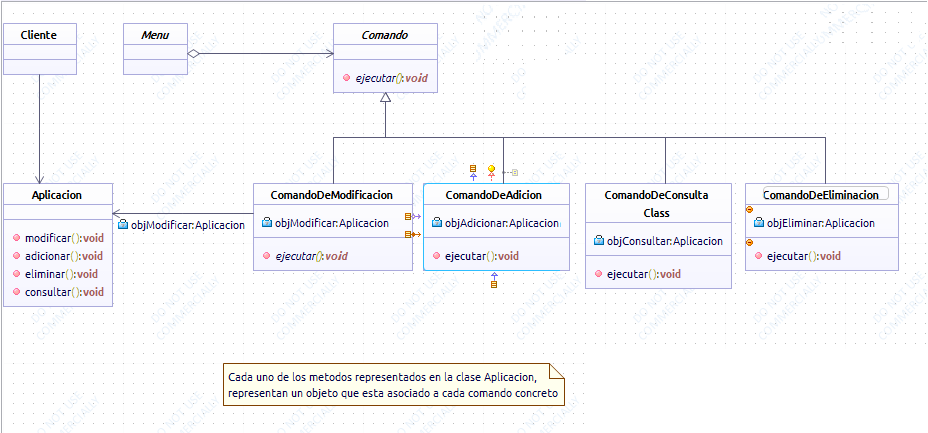
\includegraphics[width=0.6\linewidth]{ceComando}
    \centering
    \caption{Comando del sistema de gestión de tutorías.}
	\label{fig:ceComando}
\end{figure}
\indent La clave de este patrón es la clase abstracta Comando, esta declara una interfaz para ejecutar las líneas de operaciones, en este caso, esta clase tiene consigo una operación, también abstracta la cual se le suele llamar Ejecutar, con ello las subclases de orden, especifican un receptor-acción (en nuestro caso el receptor seria nuestra aplicación, por el otro lado la acción seria el comando) guardando el receptor como una variable de instancia e implementado, mientras que Ejecutar se usa para invocar la petición. Por ende, el receptor debe poseer el conocimiento necesario para llevar a cabo la petición. Una de las características y principales, y quizá la que nos da una conveniente ventaja es la de tener la posibilidad de deshacer las operaciones realizadas, también y por obvias razones buscamos independizar el momento de la petición del momento de la ejecución.
\newline

Como ya habíamos mencionado, al tener nuestra clase comando, debemos tener la especificación, es decir la clase concreta de nuestro comando, con ello nos permitimos separar tareas, y es esta clase la que conocerá la procedencia de la petición.  La clase menu será nuestra interfaz gráfica, es decir un menú con opciones desplegables sobre ciertas tareas a cumplir.Y por otro lado la clase app será la que implemente la funcionalidad real, es decir nuestra aplicación en sí, esta sera nuestra clase receptor. Podrá observar un ejemplo de su implementación en el anexo 8.1.5.
\newpage

\chapterimage{arquitectos-tenerife.jpg}
\chapter{Despliegue}

\section{Introducción}

\newpage

\section{Diagrama de Sistemas}

\newpage

\section{Diagrama de Componentes}

\newpage

\section{Diagrama de Artefactos}

\newpage

\section{Diagrama de Nodos}

\newpage



%------------------------------------------------


%----------------------------------------------------------------------------------------
%	Conclusiones
%----------------------------------------------------------------------------------------


%------------------------------------------------

\part{Conclusiones}
\chapterimage{754559_image12520430_0.jpg}
\chapter{Conlusiones}
\chapterimage{Predicciones-del-furturo-del-retail-de-moda-para-el-2020.jpg}
\chapter{Trabajos Futuros}
\chapterimage{addb4870c144badba811c06724df8512.jpg}
\chapter{Anexos}
\section{Código}
\subsection{Patrón Fachada}
\begin{figure}[H]
	\centering
	\includegraphics[width=0.5\linewidth]{codfachada1}
	\centering
	\caption{Interfaz monitoría (fachada)}
	\label{fig:codfachada1}
\end{figure}
\clearpage
\begin{figure}[H]
	\centering
	\includegraphics[width=1\linewidth]{codfachada2}
	\centering
	\caption{Ejemplo de implementación para la fachada}
	\label{fig:codfachada2}
\end{figure}
\begin{figure}[H]
	\centering
	\includegraphics[width=1\linewidth]{codfachada3}
	\centering
	\caption{Cliente ejemplo fachada}
	\label{fig:codfachada3}
\end{figure}
\subsection{Patrón Proxy}
\begin{figure}[H]
	\centering
	\includegraphics[width=0.5\linewidth]{codproxy1}
	\centering
	\caption{Clase abstracta de las bases de datos}
	\label{fig:codproxy1}
\end{figure}
\clearpage
\begin{figure}[H]
	\centering
	\includegraphics[width=0.7\linewidth]{codproxy2}
	\centering
	\caption{Clase proxy para el manejo de la conexión en SQLite}
	\label{fig:codproxy2}
\end{figure}
\begin{figure}[H]
	\centering
	\includegraphics[width=1\linewidth]{codproxy3}
	\centering
	\label{fig:codproxy3}
\end{figure}
\begin{figure}[H]

	\includegraphics[width=0.7\linewidth]{codproxy4}
	\caption{Clase con la lógica de la base de datos para SQLite}

\end{figure}
\begin{figure}[H]
	\centering
	\includegraphics[width=1\linewidth]{codproxy5}
	\centering
		\caption{Cliente con un ejemplo de implementación}
	\label{fig:codproxy5}
\end{figure}

\subsection{Patrón Comando}
\begin{figure}[H]
	\centering
	\includegraphics[width=0.5\linewidth]{codComando1}
	\centering
	\caption{Clase Cliente que ejecuta el comando}
	\label{fig:codComando1}
\end{figure}
\clearpage
\begin{figure}[H]
	\centering
	\includegraphics[width=0.7\linewidth]{codComando2}
	\centering
	\caption{Clase Aplicacion donde se manejan las consultas a la BD}
	\label{fig:codComando2}
\end{figure}
\begin{figure}[H]
	\centering
	\includegraphics[width=1\linewidth]{codComando3}
	\centering
	\caption{Interface comando}
	\label{fig:codComando3}
\end{figure}
\begin{figure}[H]
	\centering
	\caption{Implementación de la interfaz comando por cada metodo de Aplicacion}
	\includegraphics[width=1\linewidth]{codComando4}
	\caption{Comando de Modificación}
	\centering
	\label{fig:codComando4}
\end{figure}
\begin{figure}[H]
	\centering
	\includegraphics[width=1\linewidth]{codComando5}
	\centering
	\caption{Comando de Adición}
	\label{fig:codComando5}
\end{figure}
\begin{figure}[H]
	\centering
	\includegraphics[width=1\linewidth]{codComando6}
	\centering
	\caption{Comando de Eliminación}
	\label{fig:codComando6}
\end{figure}
\begin{figure}[H]
	\centering
	\includegraphics[width=1\linewidth]{codComando7}
	\centering
	\caption{Comando de Consulta}
	\label{fig:codComando7}
\end{figure}
\begin{figure}[H]
	\centering
	\includegraphics[width=1\linewidth]{codComando8}
	\centering
	\caption{Clase Menu con la que interactua el cliente en la GUI}
	\label{fig:codComando8}
\end{figure}




%----------------------------------------------------------------------------------------
%	BIBLIOGRAPHY
%----------------------------------------------------------------------------------------

\chapterimage{Libraria-Lello-_-Irmao.jpg}


\bibliographystyle{plain}
\bibliography{bibliography}



\end{document}
